\documentclass{report}
\usepackage{graphicx} % Required for inserting images
\usepackage{geometry}[margin=1in]
\usepackage{amsmath}
\usepackage{amsfonts}
\usepackage[colorlinks=true, linkcolor=black]{hyperref}
\usepackage{listings}
\usepackage{xcolor}
\usepackage{tabularx}
\usepackage{graphicx}
\usepackage{array}
\usepackage{booktabs}
\usepackage{booktabs} % For \toprule, \midrule, \bottomrule

\definecolor{codegreen}{rgb}{0,0.6,0}
\definecolor{codegray}{rgb}{0.5,0.5,0.5}
\definecolor{codepurple}{rgb}{0.58,0,0.82}
\definecolor{backcolour}{rgb}{0.95,0.95,0.92}

\lstdefinestyle{mystyle}{
    backgroundcolor=\color{backcolour},   
    commentstyle=\color{codegreen},
    keywordstyle=\color{magenta},
    numberstyle=\tiny\color{codegray},
    stringstyle=\color{codepurple},
    basicstyle=\ttfamily\footnotesize,
    breakatwhitespace=false,         
    breaklines=true,                 
    captionpos=b,                    
    keepspaces=true,                 
    numbers=left,                    
    numbersep=5pt,                  
    showspaces=false,                
    showstringspaces=false,
    showtabs=false,                  
    tabsize=2
}

\lstset{style=mystyle}

\begin{document}

\begin{titlepage}
    \centering
    
    \vspace*{1.5cm}    
    {\Huge \textbf{Summer Project Record}}\\[1cm]
    
    {\LARGE Investigations into the Fundamental Principles of Interferometric Techniques for Gravitational-Wave detection}\\[2cm]

    The optical simulations presented in this work were carried out using the Finesse 3 interferometer simulation package \cite{FinesseDocs}. The theoretical background on Michelson interferometers and gravitational-wave response follows the treatment of Bond \textit{et al.} \cite{Bond2016}. \\ [1cm]
    
    \textbf{Submitted by}\\[0.3cm]
    Rudra Sahu\\
    BS-MS Sophomore\\
    IISER Pune\\[1cm]
    
    \textbf{Under the Supervision of}\\[0.3cm]
    Deepak Pandey\\
    Associate Professor\\
    IUCAA, Pune \\[1.5cm]
    
    \textbf{Duration}\\
    May 2026 -- July 2026
    
    \vfill

    \begin{figure}[h!]
        \centering
        \includegraphics[width=0.3\linewidth]{Screenshot 2026-05-16 165051.png}
        \label{fig:placeholder}
    \end{figure}
\end{titlepage}

\tableofcontents

\newpage

\chapter{Introduction}
\section{About Gravitational Waves and Interferometry}
Gravitational waves are transverse quadrupole waves travelling at the speed of light. They are distortions in spacetime that can be detected by measuring the distance between test masses.

Gravitational waves are ripples in the fabric of spacetime produced by the acceleration of massive astrophysical objects. They were first predicted by Albert Einstein in 1916 as a consequence of the General Theory of Relativity. According to the theory, massive objects curve spacetime, and dynamic changes in this curvature propagate outward as waves travelling at the speed of light.

Astrophysical events such as binary black hole mergers, neutron star collisions, and supernova explosions generate gravitational waves of measurable amplitude. However, by the time these waves reach Earth, their effect is extremely small. The relative change they produce in distance, known as strain, is typically of the order of
\begin{equation}
h = \frac{\Delta L}{L} \sim 10^{-21}
\end{equation}

which corresponds to a displacement much smaller than the diameter of a proton over kilometre-scale distances. Detecting such tiny variations requires highly sensitive experimental techniques.

Interferometry provides one of the most effective methods for detecting gravitational waves. In an interferometer, coherent laser beams are split into two perpendicular arms and reflected using mirrors. When the beams recombine, they produce an interference pattern determined by the relative optical path lengths of the two arms.

\begin{figure}
    \centering
    \includegraphics[width=0.5\linewidth]{Screenshot 2026-05-12 230014.png}
    \caption{Simplified layout of a Michelson interferometer. The laser provides the input light, which is split into two beams by the central beamsplitters. The beams reflect off the end mirrors and recombine at the beamsplitter. The light power on the main photo detector (PD) changes when the difference between the arm length $\Delta L = L_X - L_Y$ changes.}
    \label{fig:placeholder}
\end{figure}

A passing gravitational wave stretches one arm of the interferometer while simultaneously compressing the other. This changes the relative phase of the returning laser beams, producing a measurable shift in the interference signal. Since the phase of light is extremely sensitive to path-length variations, interferometers can detect extraordinarily small spacetime distortions.

Modern gravitational wave detectors such as the \textit{Laser Interferometer Gravitational-Wave Observatory} (LIGO) employ large-scale Michelson interferometers. These detectors use high-power, stabilised lasers, ultra-high-vacuum systems, and precision mirror suspensions to minimise noise and improve measurement accuracy.

The first direct detection of gravitational waves was achieved by LIGO in 2015 from the merger of two black holes. This discovery confirmed a major prediction of General Relativity and opened a new observational window into the universe: gravitational wave astronomy.

Understanding the behaviour of interferometric systems is therefore essential for modern precision physics experiments. Numerical simulation tools such as \textit{Finesse 3} are widely used to model optical cavities, laser fields, and detector responses in gravitational wave interferometers. In this project, interferometric systems were simulated and analysed to study resonance phenomena, optical interference, and signal-generation mechanisms relevant to gravitational-wave detection.

\section{Plane-Wave Analysis}
In optical interferometry, electromagnetic waves are described using electric fields that vary in both space and time. A general expression for a paraxial light beam is given by
\begin{equation}
\vec{E}(x,y,z,t)=E_0 \vec{e}_p \cos(\omega t-\vec{k}\cdot\vec{r}+\varphi)\,U(x,y,z)
\end{equation}

where $E_0$ is the field amplitude, $\omega$ is the angular frequency, $\vec{k}$ is the wave vector, $\varphi$ is the phase offset, and $U(x,y,z)$ describes the spatial profile of the beam. The vector $\vec{e}_p$ represents the polarisation direction of the electric field.

This expression completely describes a propagating laser beam. However, for interferometric modelling, especially in the initial stages of analysis, several simplifying assumptions can be made.

\subsection{Neglecting Polarisation}

If the optical system does not contain polarising elements such as waveplates or polarising beam splitters, the polarisation state of the beam does not significantly affect the analysis. The vector nature of the electric field can therefore be ignored:
\begin{equation}
\vec{e}_p \rightarrow 1,
\qquad
\vec{E} \rightarrow E
\end{equation}

This reduces the electric field from a vector quantity to a scalar quantity.

\subsection{Alignment Along the Beam Axis}

The coordinate system is chosen such that the laser beam propagates along the $z$-axis. Under this condition,
\begin{equation}
\vec{k}\cdot\vec{r}=kz,
\quad
\text{where}
\quad
k=\frac{\omega}{c}=\frac{2\pi}{\lambda}
\end{equation}
is the magnitude of the wave vector. The electric field expression then becomes
\begin{equation}
E = E_0 \cos(\omega t-kz+\varphi)\,U(x,y,z)
\end{equation}

\subsection{Plane Wave Approximation}

To further simplify the analysis, the spatial beam profile is assumed to be ignored.
\begin{equation}
U(x,y,z)=1
\end{equation}

This assumption removes all dependence on the transverse coordinates $x$ and $y$. Physically, this corresponds to an idealised beam with infinite transverse extent and a uniform intensity distribution. Such a wave is called a \textit{plane wave}.

Although real laser beams possess finite beam widths and Gaussian intensity profiles, the plane wave approximation is extremely useful because it captures the essential phase and propagation behaviour relevant to interferometry.

Applying all these simplifications gives the final plane wave expression:
\begin{equation}
E = E_0 \cos(\omega t-kz+\varphi)
\end{equation}

This equation describes a monochromatic electromagnetic wave propagating in the positive $z$-direction. The phase term $(\omega t-kz+\varphi)$ determines the oscillatory behaviour of the field and plays a central role in interference phenomena.

In interferometric gravitational wave detectors, the relative phase difference between optical fields travelling through different paths determines the detector output signal. Consequently, even this simplified plane wave description provides a powerful foundation for understanding optical interference and cavity resonance behaviour.

\section{Photodetection and Optical Power}

In interferometric systems, optical signals are measured by photodiodes. A photodiode converts incident optical power into an electrical signal. Importantly, photodiodes do not directly measure the electric field of light; instead, they respond to the intensity of the electromagnetic wave.

For an electromagnetic wave, the intensity is proportional to the square of the electric field amplitude. The optical power incident on a detector is therefore obtained by integrating the intensity over the cross-sectional area of the beam:
\begin{equation}
P = \iint I(x,y,z_0)\,dx\,dy
\end{equation}

where $z_0$ represents the position of the photodiode along the propagation axis. The intensity of the electromagnetic field is given by
\begin{equation}
I = c\varepsilon_0 E^2
\end{equation}

where $c$ is the speed of light and $\varepsilon_0$ is the permittivity of free space.

Using the plane wave expression for the electric field,
$E = E_0 \cos(\omega t)$, the detected optical power becomes
\begin{equation}
P = c\varepsilon_0 E_0^2 \cos^2(\omega t)
\end{equation}

Applying the trigonometric identity
$\cos^2(\omega t)=\frac{1}{2}\left(1+\cos(2\omega t)\right)$
gives
\begin{equation}
P = \frac{c\varepsilon_0}{2}E_0^2\left(1+\cos(2\omega t)\right)
\end{equation}

The second term oscillates at a frequency $2\omega$, which is twice the laser's optical frequency. For visible and infrared laser light, $\omega$ is typically of the order of $10^{15}\,\text{Hz}$. Such rapid oscillations are far beyond the response bandwidth of ordinary photodiodes and electronic circuits.

As a result, the detector effectively averages the rapidly oscillating term over time: 
$\left\langle \cos(2\omega t) \right\rangle = 0$
, and the measured optical power reduces to
\begin{equation}
\boxed{P = \frac{c\varepsilon_0}{2}E_0^2}
\end{equation}

Thus, the detected signal appears constant for a single monochromatic optical field.

\section{Complex Representation of Optical Fields}

In interferometry and optical simulations, it is often convenient to describe electromagnetic fields using complex notation rather than purely real trigonometric functions. This mathematical representation significantly simplifies calculations involving phase shifts, interference, and propagation through optical systems.

The real electric field of a monochromatic plane wave is written as

\begin{equation}
E'(z,t)=E_0' \cos(\omega t-kz+\varphi)
\end{equation}

where $E_0'$ is the real field amplitude, $\omega$ is the angular frequency, $k$ is the wave number, and $\varphi$ is the phase offset.

Using Euler's relation,
$e^{i\theta}=\cos\theta+i\sin\theta$
the field can instead be represented in complex form as
\begin{equation}
E(z,t)=E_0 e^{i(\omega t-kz)}
\end{equation}

where the complex amplitude is defined as
$E_0 = E_0' e^{i\varphi}$
. In this notation, the phase information is incorporated directly into the complex amplitude.

The physical electric field is obtained by taking only the real part of the complex expression:
\begin{equation}
E'(z,t)=\Re\{E(z,t)\}
\end{equation}

The complex field itself does not represent a physically measurable quantity. Instead, it is a mathematical tool that simplifies optical calculations.

One major advantage of this formalism is that phase changes become simple multiplicative operations. For example, if an optical field acquires an additional phase shift $\phi$ while propagating through an optical component, the field transforms as
$E \rightarrow E e^{i\phi}$

This property greatly simplifies the modelling of interferometers, especially in numerical simulation packages such as \textit{Finesse 3}, where mirrors, beam splitters, and cavities primarily modify the amplitude and phase of optical fields.

To further simplify calculations, a constant factor of
$\sqrt{c\varepsilon_0/2}$
is absorbed into the field amplitude definition. As a result, the amplitude $E_0$ acquires units of $\sqrt{\text{W}}$, allowing optical power to be written directly as
\begin{equation}
P = E_0 E_0^* = |E_0|^2
\end{equation}

where $E_0^*$ denotes the complex conjugate of the field amplitude.

The final form of the optical field therefore becomes
$\boxed{E(z,t)=E_0 e^{i(\omega t-kz)}}$, with optical power given by
$\boxed{P=|E_0|^2}$


\chapter{Optical Interactions with Components}
In an interferometric system, laser beams propagate through a network of optical components, including mirrors, beam splitters, lenses, modulators, and cavities. Each component modifies the amplitude, phase, direction, or frequency content of the optical field. The term \textit{optical surface} generally refers to a boundary between two media with possibly different indices of refraction $n$.

\section{Propagation Through Free Space}

As an optical field propagates through free space, it accumulates a phase proportional to the distance travelled. Although the amplitude of the field remains unchanged in an ideal lossless medium, the propagation introduces a phase delay that plays a central role in interference phenomena.

\begin{figure}[h!]
    \centering
    \includegraphics[width=0.3\linewidth]{Screenshot 2026-05-13 215904.png}
    \caption{Coupling of field amplitudes for free propagation}
    \label{fig:placeholder}
\end{figure}

Consider an optical field travelling through a space of length $L$. Using the complex field formalism, the propagation of the field is represented by a multiplicative phase factor:

\begin{equation}
a_2 = a_1 e^{-ikL}
\end{equation}

Similarly, for light propagating in the opposite direction,

\begin{equation}
a_4 = a_3 e^{-ikL}
\end{equation}

where $a_1$ and $a_3$ are the incident complex field amplitudes, while $a_2$ and $a_4$ are the corresponding propagated fields.

\section{Mirror}
A mirror partially reflects and partially transmits an incident optical field. Let $r$ denote the amplitude reflectivity and $t$ denote the amplitude transmissivity of the mirror.

\begin{figure}[h!]
    \centering
    \includegraphics[width=0.17\linewidth]{Screenshot 2026-05-13 221444.png}
    \caption{Coupling of field amplitudes at a mirror}
    \label{fig:placeholder}
\end{figure}

If $a_1$ and $a_3$ are the incoming optical fields on either side of the mirror, the outgoing fields $a_2$ and $a_4$ are given by

\begin{equation}
a_2 = r a_3 + i t a_1
\end{equation}
\begin{equation}
a_4 = r a_1 + i t a_3
\end{equation}

The reflected fields acquire the factor $r$, while the transmitted fields acquire the factor $it$. The factor of $i$ corresponds to a phase shift of $\pi/2$ introduced during transmission. This phase convention ensures energy conservation and consistent interference behaviour within interferometric systems.

For a lossless mirror,

\begin{equation}
|r|^2 + |t|^2 = 1
\end{equation}

\section{Beam Splitter}

A beam splitter functions similarly to a partially transmitting mirror, but it couples four optical ports simultaneously. In a Michelson interferometer, the beam splitter divides the incoming laser beam into two perpendicular paths and later recombines them to produce interference.

\begin{figure}[!ht]
    \centering
    \includegraphics[width=0.17\linewidth]{Screenshot 2026-05-13 221515.png}
    \caption{Caption}
    \label{fig:placeholder}
\end{figure}

The coupling relations for the beam splitter are

\begin{equation}
a_2 = r a_1 + it a_7
\end{equation}
\begin{equation}
a_4 = r a_7 + it a_1
\end{equation}
\begin{equation}
a_6 = r a_5 + it a_3
\end{equation}
\begin{equation}
a_8 = r a_3 + it a_5
\end{equation}

where the fields $a_1$, $a_3$, $a_5$, and $a_7$ represent the incident fields at different ports, while $a_2$, $a_4$, $a_6$, and $a_8$ are the corresponding outgoing fields.

For a 50:50 beam splitter,

\begin{equation}
|r|^2 = |t|^2 = \frac{1}{2}
\end{equation}

\section{Coupling Matrices for Optical Components}

The behaviour of optical systems can be described systematically using coupling matrices. Each optical component transforms the incoming field amplitudes into outgoing fields through linear matrix operations.

\subsection{Space Propagation Matrix}

Propagation through free space introduces a phase shift proportional to the propagation distance $L$. The coupling relation is

\begin{equation}
a_{\text{out}} = a_{\text{in}} e^{-ikL}
\end{equation}

which can be written in matrix form as

\begin{equation}
\begin{pmatrix}
a_2\\
a_4
\end{pmatrix}
=
\begin{pmatrix}
e^{-ikL} & 0\\
0 & e^{-ikL}
\end{pmatrix}
\begin{pmatrix}
a_1\\
a_3
\end{pmatrix}
\end{equation}

The diagonal matrix elements represent phase accumulation during propagation.

\subsection{Mirror Coupling Matrix}

The mirror interaction can be represented as

\begin{equation}
\begin{pmatrix}
a_2\\
a_4
\end{pmatrix}
=
\begin{pmatrix}
it & r\\
r & it
\end{pmatrix}
\begin{pmatrix}
a_1\\
a_3
\end{pmatrix}
\end{equation}

This matrix describes the redistribution of optical fields due to reflection and transmission at the mirror surface.

\subsection{Beam Splitter Coupling Matrix}

The beam splitter couples four ports simultaneously. Its behaviour can be represented using a larger coupling matrix relating all input and output fields:

\begin{equation}
\begin{pmatrix}
a_2\\
a_4\\
a_6\\
a_8
\end{pmatrix}
=
\begin{pmatrix}
r & 0 & 0 & it\\
it & 0 & 0 & r\\
0 & it & r & 0\\
0 & r & it & 0
\end{pmatrix}
\begin{pmatrix}
a_1\\
a_3\\
a_5\\
a_7
\end{pmatrix}
\end{equation}

\section{Phase Relationships in Reflection and Transmission}

When an electromagnetic wave encounters the boundary between two optical media, part of the wave is reflected while the remaining portion is transmitted. In addition to changes in amplitude, the reflected and transmitted fields may also acquire phase shifts. These phase relationships are fundamentally described by the Fresnel equations.

\subsection{Fresnel Equations}

Consider an optical wave incident normally on an interface separating two media with refractive indices $n_1$ and $n_2$. The Fresnel equations give the amplitude reflection and transmission coefficients as

\begin{equation}
r = \frac{n_1-n_2}{n_1+n_2}
\end{equation}

and

\begin{equation}
t = \frac{2n_1}{n_1+n_2}
\end{equation}

The coefficient $r$ determines the amplitude and phase of the reflected wave, while $t$ determines the transmitted field amplitude.

An important feature of the Fresnel reflection coefficient is its sign. If light reflects from a medium of lower refractive index to a higher refractive index $(n_2 > n_1)$, then

\begin{equation}
r < 0
\end{equation}

which corresponds to a phase shift of $\pi$ radians in the reflected field.

Conversely, when light reflects from a higher refractive index medium to a lower refractive index medium,

\begin{equation}
r > 0
\end{equation}

and no additional phase inversion occurs.

Thus, reflection can introduce relative phase shifts depending on the optical boundary conditions. These phase shifts are critically important in interference and cavity resonance phenomena.

\subsection{Phase Conventions in Interferometry}

In interferometer modelling, phase conventions are introduced to ensure mathematical consistency and energy conservation when combining reflected and transmitted fields. Two commonly used conventions are the \textit{symmetric convention} and the \textit{antisymmetric convention}.

\subsection{Antisymmetric Convention}

In conventional optics, the antisymmetric convention is closely connected to the physical phase behaviour predicted by the Fresnel equations at optical boundaries. When light reflects from an interface separating two media, the reflected field may undergo a phase change depending on the relative optical densities of the media. If the second medium is optically denser than the first, the reflected wave experiences a phase reversal of $180^\circ$. In contrast, reflection from an optically thinner medium introduces no phase inversion. Thus, the phase shift upon reflection is either $0^\circ$ or $180^\circ$ depending on the nature of the interface. Fresnel analysis further shows that, for a lossless optical surface, the transmitted field does not acquire an additional phase shift at the boundary itself. The antisymmetric convention incorporates these physical phase relationships directly into the field representation through relative sign changes between reflected and transmitted components, making it a natural framework in classical and conventional optical analysis.

\subsection{Symmetric Convention}

In the symmetric convention, both transmitted fields acquire an identical phase factor of $i$, corresponding to a phase shift of $\pi/2$:

This convention treats both transmission directions equivalently and is commonly used in interferometer simulation software such as \textsc{Finesse 3} because of its mathematical simplicity.

The factor of $i$ ensures that the optical component remains unitary for a lossless system, preserving total optical power.

\subsection{Phase Constraints}

The phase relationships associated with reflection and transmission can be understood by analysing a Michelson interferometer containing a beam splitter and two perfectly reflecting mirrors. The beam splitter acts as the optical element under investigation. The magnitudes of the amplitude reflection and transmission coefficients are assumed to be known, while the corresponding phase changes introduced during reflection and transmission are treated as unknown quantities.

\begin{figure}[h!]
    \centering
    \includegraphics[width=0.5\linewidth]{Screenshot 2026-05-13 230429.png}
    \caption{The relation between the phase of the light field amplitudes at a beam splitter can be computed assuming a Michelson interferometer,with arbitrary arm length but perfectly-reflecting mirrors. The incoming field $E_0$ is split into two fields $E_1$ and $E_2$ which are reflected at the end mirrors and return to the beam splitter, as $E3$ and $E4$, to be recombined into two outgoing fields. These outgoing fields $E5$ and $E6$ are depicted by two arrows to highlight that these are the sum of the transmitted and reflected components of the returning fields.}
    \label{fig:placeholder}
\end{figure}

Due to symmetry, the phase shift associated with transmission through the beam splitter is assumed to be identical in both propagation directions. However, the reflected field may acquire different phases depending on whether reflection occurs from the front or back surface of the beam splitter. These are denoted by $\phi_{r1}$ and $\phi_{r2}$ respectively.

The electric fields immediately after the first interaction with the beam splitter are therefore written as
\begin{equation}
E_1 = rE_0 e^{i\phi_{r1}}
\end{equation}

\begin{equation}
E_2 = tE_0 e^{i\phi_t}
\end{equation}
where $E_0$ is the incident optical field.

The lengths of the interferometer arms are generally not identical. Consequently, additional propagation phases accumulate in each arm. Let $\Phi_1$ denote the total phase accumulated in the vertical arm and $\Phi_2$ denote the total phase accumulated in the horizontal arm. After reflection from the end mirrors and propagation back to the beam splitter, the returning fields become
\begin{equation}
E_3 = rE_0 e^{i(\phi_{r1}+\Phi_1)}
\end{equation}

\begin{equation}
E_4 = tE_0 e^{i(\phi_t+\Phi_2)}
\end{equation}

The outgoing fields are obtained by summing the reflected and transmitted components at the beam splitter. This gives
\begin{equation}
E_5 = E_0 \left(
Re^{i(2\phi_{r1}+\Phi_1)}
+
Te^{i(2\phi_t+\Phi_2)}
\right)
\end{equation}
and
\begin{equation}
E_6 = E_0 rt \left(
e^{i(\phi_t+\phi_{r1}+\Phi_1)}
+
e^{i(\phi_t+\phi_{r2}+\Phi_2)}
\right)
\end{equation}
where
\begin{equation}
R=r^2,
\qquad
T=t^2
\end{equation}

represent the power reflectivity and transmissivity respectively.

To simplify the expressions, the phase factors are separated into common and differential components. The field $E_5$ can be written as
\begin{equation}
E_5
=
E_0 e^{i\alpha_+}
\left(
Re^{i\alpha_-}
+
Te^{-i\alpha_-}
\right)
\end{equation}
where
\begin{equation}
\alpha_+
=
\phi_{r1}
+
\phi_t
+
\frac{1}{2}(\Phi_1+\Phi_2)
\quad \text{and} \quad
\alpha_-
=
\phi_{r1}
-
\phi_t
+
\frac{1}{2}(\Phi_1-\Phi_2)
\end{equation}

Similarly, the second output field becomes
\begin{equation}
E_6
=
E_0 rt e^{i\beta_+}
2\cos(\beta_-)
\end{equation}
with
\begin{equation}
\beta_+
=
\phi_t
+
\frac{1}{2}
(
\phi_{r1}
+
\phi_{r2}
+
\Phi_1
+
\Phi_2
)
\quad \text{and} \quad
\beta_-
=
\frac{1}{2}
(
\phi_{r1}
-
\phi_{r2}
+
\Phi_1
-
\Phi_2
)
\end{equation}

For a 50:50 beam splitter, $r=t=\frac{1}{\sqrt{2}}$ which simplifies the output fields to
\begin{equation}
E_5
=
E_0 e^{i\alpha_+}\cos(\alpha_-)
\quad \text{and} \quad
E_6
=
E_0 e^{i\beta_+}\cos(\beta_-)
\end{equation}

Since the beam splitter is assumed to be lossless, conservation of energy requires that the total output power equal the input power:

\begin{equation}
|E_0|^2
=
|E_5|^2
+
|E_6|^2
\end{equation}

Substituting the field expressions gives

\begin{equation}
\cos^2(\alpha_-)
+
\cos^2(\beta_-)
=
1
\end{equation}

This condition is satisfied only if

\begin{equation}
\alpha_-
-
\beta_-
=
(2N+1)\frac{\pi}{2}
\end{equation}

where $N$ is any integer.

Substituting the definitions of $\alpha_-$ and $\beta_-$ yields the important phase constraint

\begin{equation}
\boxed{\frac{1}{2}
(
\phi_{r1}
+
\phi_{r2}
)
-
\phi_t
=
(2N+1)\frac{\pi}{2}}
\end{equation}

In practical interferometric calculations, the exact reflection and transmission phase factors are often neither directly measurable nor particularly important. What matters is that the chosen phase conventions satisfy the physical constraints imposed by energy conservation and interference behaviour. Consequently, it is common to adopt a mathematically convenient set of phase factors that fulfils the required phase relation for a lossless beam splitter.

In this work, the symmetric convention is used, where the transmission phase shift is chosen as $\phi_t=\frac{\pi}{2}$ while the reflection phase shift is taken to be $\phi_r=0$. Under this convention, the reflected and transmitted optical fields are written as

\begin{equation}
E_{\text{refl}} = rE_0 \quad \text{and} \quad E_{\text{trans}} = itE_0
\end{equation}

where $r$ and $t$ are positive real amplitude coefficients satisfying
\begin{equation}
r^2+t^2=1
\end{equation}
for a lossless optical component.

The factor of $i$ associated with transmission corresponds to a phase shift of $\pi/2$. This choice satisfies the phase constraint derived from the Michelson interferometer analysis and ensures that the optical system conserves energy. Importantly, this convention introduces a symmetric mathematical representation for mirrors and beam splitters.

One major advantage of the symmetric convention is that it avoids the need to distinguish explicitly between front and back surfaces of optical components. The coupling relations remain identical regardless of propagation direction, which greatly simplifies matrix-based interferometric calculations.

\section{Macroscopic Length and Microscopic Tuning}

In interferometric optical systems, the resonance condition depends not on the absolute distance between optical components, but on the optical path length modulo the laser wavelength. For laser light with a wavelength of the order of $\lambda \approx 1\ \mu\text{m}$, only length variations comparable to the wavelength significantly affect interference and resonance conditions.

For example, in the arm cavities of the Virgo gravitational wave detector, the cavity length is approximately  $L \approx 3\ \text{km}$ while the laser wavelength is nearly a million times smaller. If one mirror is displaced by $\Delta x = \frac{\lambda}{2}$, the optical field acquires an additional round-trip phase shift of $2\pi$, recreating exactly the same resonance condition inside the cavity.

However, many global cavity properties such as the free spectral range and finesse depend on the large-scale cavity length and are essentially unchanged by microscopic displacements on the order of a wavelength. This naturally separates the optical system into two different length scales:
\begin{itemize}
    \item a \textbf{macroscopic length}, determining the overall cavity geometry,
    \item a \textbf{microscopic tuning}, determining the interference condition.
\end{itemize}

To improve both physical interpretation and numerical accuracy, the total distance $D$ between two optical components is therefore written as
\begin{equation}
D = L + T
\end{equation}

where:

\begin{itemize}
    \item $L$ is the macroscopic length, chosen as an integer multiple of a reference wavelength $\lambda_0$,
    \item $T$ is the microscopic tuning, representing the remaining small displacement.
\end{itemize}

Propagation through a distance $D$ introduces a phase shift
\begin{equation}
\phi = -kD
\end{equation}

Writing the optical frequency as $\omega=\omega_0+\Delta\omega$ and substituting $D=L+T$, the phase becomes
\begin{equation}
-\phi
=
\frac{\omega_0 L}{c}
+
\frac{\Delta\omega L}{c}
+
\frac{\omega_0 T}{c}
+
\frac{\Delta\omega T}{c}
\end{equation}

The first term is always an integer multiple of $2\pi$ and therefore has no physical effect on interference. The last term is typically extremely small and can usually be neglected. The dominant contributions are therefore
\begin{equation}
\phi
\approx
-
\frac{\Delta\omega L}{c}
+
\frac{\omega_0 T}{c}
\end{equation}

It is convenient to define the microscopic tuning directly as a phase:
\begin{equation}
\varphi=\frac{\omega_0 T}{c}
\end{equation}

giving the final expression
\begin{equation}
\boxed{\phi
\approx
-
\frac{\Delta\omega L}{c}
+
\varphi}
\end{equation}

This convention greatly improves numerical precision in interferometric simulations. The macroscopic length $L$ describes large-scale propagation through free space, while the tuning $\varphi$ effectively represents microscopic mirror displacement and determines the resonance condition of the interferometer.

\section{Tuning a Beamsplitter using Finesse 3}
\begin{lstlisting}[language=python]
from finesse import Model
from finesse.analysis.actions import Xaxis
import matplotlib.pyplot as plt
import numpy as np

# ================== SWEEP MICROSCOPIC TUNING ========================
model_phi = Model()

model_phi.parse("""
l l1 P=1   # Laser
s s1 l1.p1 b1.p1 L=1     # First space
bs b1 R=1 T=0 alpha=0    # Beam splitter acting as turning mirror
s s2 b1.p2 dump.p1 L=1   # Second space
m dump R=1 T=0           # Dummy sink 
ad ad1 dump.p1.i 0       # Dummy sink
""")

out_phi = model_phi.run(Xaxis(parameter="b1.phi", mode="lin", start=0, stop=180, steps=100))
phase_phi = np.angle(out_phi["ad1"], deg=True)

# ================== SWEEP MACROSCOPIC LENGTH ========================
model_L = Model()

model_L.parse("""
l l1 P=1                 # Laser
s s1 l1.p1 b1.p1 L=1     # First space
bs b1 R=1 T=0 alpha=0    # Beam splitter
s s2 b1.p2 dump.p1 L=1   # Second space
m dump R=1 T=0           # Dummy sink
ad ad1 dump.p1.i 0       # Amplitude detector
""")

out_L = model_L.run(Xaxis(parameter="s1.L", mode="lin", start=1, stop=2, steps=100))
phase_L = np.angle(out_L["ad1"], deg=True)

# ======================== PLOTTING ==========================
fig, axs = plt.subplots(1,2, figsize=(12,5))
# ------------------------------------------------------------
axs[0].plot(out_phi.x[0], phase_phi)
axs[0].set_xlabel("Beam Splitter Tuning $\phi$ [deg]")
axs[0].set_ylabel("Optical Phase [deg]")
axs[0].set_title("Phase vs Microscopic Tuning")
axs[0].grid(True)
# ------------------------------------------------------------
axs[1].plot(out_L.x[0], phase_L)
axs[1].set_xlabel("Space Length L [m]")
axs[1].set_ylabel("Optical Phase [deg]")
axs[1].set_title("Phase vs Macroscopic Length")
axs[1].grid(True)

plt.tight_layout()
plt.show()
\end{lstlisting}
\begin{figure}[h!]
    \centering
    \includegraphics[width=\linewidth]{image.png}
    \caption{(a) The phase change of a beam reflected by a beam splitter as a function of the beam splitter tuning. (b)  if a length of a space is changed, the phase of the transmitted light isunchanged (for the default wavelength $\Delta k = 0$)}
    \label{fig:placeholder}
\end{figure}
\section{Revised Coupling Matrices for Spaces and Mirrors}

Using the definitions of macroscopic length and microscopic tuning, the coupling relations for optical components can be rewritten in a more numerically stable and physically meaningful form. In this convention, the large propagation distance is separated from the microscopic phase tuning associated with the optical components.
\begin{figure}[h!]
    \centering
    \includegraphics[width=0.3\linewidth]{Screenshot 2026-05-16 153939.png}
    \caption{Tuning the mirror}
    \label{fig:placeholder}
\end{figure}
For a mirror, the coupling equations are modified such that the microscopic tuning appears explicitly as a phase factor associated with the optical surface. The reflected and transmitted fields are therefore written as
\begin{equation}
\begin{pmatrix}
a_2 \\
a_4
\end{pmatrix}
=
\begin{pmatrix}
r e^{i\phi} & it \\
it & r e^{-i\phi}
\end{pmatrix}
\begin{pmatrix}
a_3 \\
a_1
\end{pmatrix}
\end{equation}
where $\phi$ represents the microscopic tuning of the mirror.

The propagation through free space is described only through the macroscopic length $L$. The corresponding coupling relations become
\begin{equation}
\begin{pmatrix}
a_2 \\
a_4
\end{pmatrix}
=
\begin{pmatrix}
e^{-i\frac{\Delta\omega L}{c}} & 0 \\
0 & e^{-i\frac{\Delta\omega L}{c}}
\end{pmatrix}
\begin{pmatrix}
a_1 \\
a_3
\end{pmatrix}
\end{equation}
where $\Delta\omega$ is the frequency offset relative to the reference optical frequency.

In practical interferometer modelling, this convention also simplifies the interpretation of cavity resonance conditions. The resonance behaviour is controlled entirely through the tuning parameters of the mirrors, while the macroscopic cavity length determines quantities such as the free spectral range.

\chapter{The Fabry-P\'erot Etalon}
It is an optical cavity made from two parallel reflecting surfaces (i.e., thin mirrors). Optical waves can pass through the optical cavity only when they are in resonance with it.

\begin{figure}[h!]
    \centering
    \includegraphics[width=0.4\linewidth]{Screenshot 2026-05-13 231955.png}
    \caption{Setup of a Fabry-P\'erot Interferometer}
    \label{fig:placeholder}
\end{figure}

\section{Field Relations in a Fabry--P\'erot Cavity}

The cavity is defined by a propagation length $L$ in vacuum, amplitude reflectivities $r_1$ and $r_2$, and amplitude transmittivities $t_1$ and $t_2$ for the two mirrors. The optical field amplitudes at different points inside the cavity can be obtained through the superposition of reflected and transmitted fields.

The complete set of field equations for the cavity is given by
\begin{align}
a_1 &= it_1 a_0 + r_1 a_3' \\
a_1' &= e^{-ikL} a_1 \\
a_2 &= it_2 a_1' \\
a_3 &= r_2 a_1' \\
a_3' &= e^{-ikL} a_3 \\
a_4 &= r_1 a_0 + it_1 a_3'
\end{align}

The circulating field incident on the first mirror surface, $a_3'$, can be computed as

\begin{align}
a_3'= e^{-ikL} a_3 = e^{-ikL} r_2 a_1'= e^{-i2kL} r_2 a_1 = e^{-i2kL} r_2 \left( it_1 a_0 + r_1 a_3' \right)
\end{align}

Solving for $a_3'$ gives
\begin{equation}
a_3'
=
a_0
\frac{
i r_2 t_1 e^{-i2kL}
}{
1-r_1 r_2 e^{-i2kL}
}
\end{equation}

The reflected field from the cavity is then obtained as
\begin{equation}
    \boxed{a_4=a_0\frac{r_1-r_2(r_1^2+t_1^2)e^{-i2kL}}{1-r_1 r_2 e^{-i2kL}}}
\end{equation}

while the transmitted field becomes

\begin{equation}
\boxed{a_2=a_0\frac{-t_1 t_2 e^{-ikL}}{1-r_1 r_2 e^{-i2kL}}}
\end{equation}

\section{Cavity Transfer Function and Resonance Properties}

The transmission behaviour of a Fabry--P\'erot cavity can be described through the ratio of the transmitted optical field to the injected field. If $a_0$ represents the input field and $a_2$ represents the transmitted field, then the frequency-dependent transfer function of the cavity in transmission is

\begin{equation}
\frac{a_2}{a_0}
=
\frac{
-t_1 t_2 e^{-ikL}
}{
1-r_1 r_2 e^{-i2kL}
}
\end{equation}

The frequency dependence enters through the wave number

\begin{equation}
k=\frac{2\pi f}{c}
\end{equation}

where $f$ is the laser frequency and $c$ is the speed of light.

The circulating optical power inside the cavity depends strongly on the laser frequency. Maximum intracavity power occurs when the denominator of the cavity response becomes minimum. This happens when the round-trip phase accumulated by the optical field is an integer multiple of $2\pi$. The resonance condition is therefore

\begin{equation}
2L = N\lambda
\end{equation}

where $N$ is an integer and $\lambda$ is the wavelength of the injected light.

Using the relation, $k=\frac{2\pi}{\lambda}$ the resonance condition can be rewritten as
\begin{equation}
2L = \frac{N2\pi}{k} \quad \implies \quad \boxed{kL = N\pi}
\end{equation}

Minimum circulating power occurs at anti-resonance, where
\begin{equation}
kL = \left(N+\frac{1}{2}\right)\pi
\end{equation}
corresponding to destructive interference between successive round-trip fields.

\begin{figure}[h!]
    \centering
    \includegraphics[width=0.7\linewidth]{Screenshot 2026-05-13 234637.png}
    \caption{Power enhancement in a two-mirror cavity as a function of the laser-light frequency. The peaks marks the resonances of the cavity,i.e., modes of operation in which the injected light is resonantly enhanced.}
    \label{fig:placeholder}
\end{figure}
\subsection{Free Spectral Range}
The phase accumulated during a round trip can also be written as

\begin{equation}
2kL
=
\frac{\omega 2L}{c}
=
2\pi f \frac{2L}{c}
=
2\pi \frac{f}{\text{FSR}}
\end{equation}

where the quantity
\begin{equation}
\boxed{\text{FSR}=\frac{c}{2L}}
\end{equation}
is called the \textit{free spectral range} of the cavity.

The free spectral range represents the frequency spacing between adjacent cavity resonances. Resonance therefore occurs at frequencies
\begin{equation}
f_r = N\cdot \text{FSR}
\end{equation}
with $N$ being an integer.

\subsection{Linewidth}
Another important characteristic of the cavity is its linewidth, usually specified by its full width at half maximum (FWHM) or equivalently by the pole frequency $f_p$. The linewidth is determined by the frequency at which the circulating power falls to half of its maximum value. This yields the full linewidth expression
\begin{equation}
\boxed{\text{FWHM}
=
2f_p
=
\frac{2\text{FSR}}{\pi}
\arcsin
\left(
\frac{1-r_1 r_2}{2\sqrt{r_1 r_2}}
\right)}
\end{equation}

\subsection{Finesse}
The ratio of the free spectral range to the linewidth defines the cavity finesse:
\begin{equation}
\boxed{\mathcal{F}
=
\frac{\text{FSR}}{\text{FWHM}}
=
\frac{\pi}{
2\arcsin
\left(
\frac{1-r_1 r_2}{2\sqrt{r_1 r_2}}
\right)
}}
\end{equation}
The finesse of a cavity is its quality factor. The finesse measures the sharpness of the cavity resonance peaks. High finesse cavities exhibit narrow resonances and large intracavity power buildup.

For highly reflective mirrors where
\begin{equation}
r_1 \approx 1,
\qquad
r_2 \approx 1
\end{equation}
the argument of the arcsine function becomes small, allowing the approximation
\begin{equation}
\mathcal{F}
\approx
\frac{\pi\sqrt{r_1 r_2}}{1-r_1 r_2}
\approx
\frac{\pi}{1-r_1 r_2}
\end{equation}

The optical behaviour of a two-mirror cavity depends strongly on the reflectivities of the mirrors. Three important coupling regimes are commonly identified:
\begin{itemize}
    \item \textbf{Undercoupled cavity:}
    \begin{equation}
    T_1 < T_2
    \end{equation}
    
    \item \textbf{Impedance matched cavity:}
    \begin{equation}
    T_1 = T_2
    \end{equation}
    
    \item \textbf{Overcoupled cavity:}
    \begin{equation}
    T_1 > T_2
    \end{equation}
\end{itemize}
where $T_1$ and $T_2$ are the mirror power transmissivities.

These coupling regimes determine how efficiently light enters the cavity and how much power is reflected or transmitted. Fabry--P\'erot cavities with carefully chosen parameters are essential components in high-precision interferometric systems, including gravitational wave detectors.

\section{Simulating Fabry-P\'erot Cavity using Finesse 3}

\begin{lstlisting}[language=Python]
import numpy as np
from finesse import Model
from finesse.analysis.actions import Xaxis
import matplotlib.pyplot as plt
from matplotlib.ticker import MaxNLocator

model = Model()

model.parse("""
l laser P=1  # Laser (Power = 1 W)
s s1 laser.p1 m1.p1 L=1    # Space (Length = 1 m)

m m1 R=0.9 T=0.1
s sL m1.p2 m2.p1 L=2000
m m2 R=0.9 T=0.1

# Photo diodes measuring DC-power
pd refl m1.p1.o
pd circ m1.p2.i
pd tran m2.p2.o           
""")

# Running the frequency sweep
out3 = model.run(
    Xaxis(
        parameter="laser.f",
        mode="lin",
        start=-100e3,
        stop=100e3,
        steps=400
    )
)

# Plot
fig, ax = plt.subplots(1, 3, figsize=(15,5))

# ---------------- Reflection ----------------
ax[0].plot(out3.x[0], out3["refl"])
ax[0].set_title("Reflection")
ax[0].set_xlabel("Frequency Offset [Hz]")
ax[0].set_ylabel("Power [W]")
ax[0].grid(True)

# ---------------- Circulation ----------------
ax[1].plot(out3.x[0], out3["circ"])
ax[1].set_title("Circulating Power")
ax[1].set_xlabel("Frequency Offset [Hz]")
ax[1].set_ylabel("Power [W]")
ax[1].set_yscale("log")
ax[1].grid(True)

# ---------------- Transmission ----------------
ax[2].plot(out3.x[0], out3["tran"])
ax[2].set_title("Transmission")
ax[2].set_xlabel("Frequency Offset [Hz]")
ax[2].set_ylabel("Power [W]")
ax[2].set_yscale("log")
ax[2].grid(True)

for a in ax:
    a.set_xlabel("Frequency Offset [Hz]")
    a.set_ylabel("Power [W]")
    a.grid(True)
    a.xaxis.set_major_locator(MaxNLocator(6)) 
    
fig.suptitle("Fabry-Perot Cavity Response", fontsize=16)
plt.tight_layout()
plt.show()

c = 3e8   # speed of light (m/s)
L = 2000   # cavity length (m)
R1 = 0.9
R2 = 0.9
FSR = c / (2 * L)  #FSR
F = (np.pi * np.sqrt(R1 * R2)) / (1 - R1 * R2)  # Finesse
linewidth = FSR / F   # Linewidth

print(f"FSR       = {FSR:.2f} Hz")
print(f"Finesse   = {F:.2f}")
print(f"Linewidth = {linewidth:.2f} Hz")
\end{lstlisting}

\begin{figure}[h!]
    \centering
    \includegraphics[width=\linewidth]{output.png}
    \caption{Output plots with FSR = 75000.00 Hz, Finesse = 14.88 and Linewidth = 5039.91 Hz}
    \label{fig:placeholder}
\end{figure}

\chapter{Modulation of Light Fields}

In interferometric systems, information is transmitted by encoding a signal onto a high-frequency optical carrier wave. The laser field serves as the carrier, while physical signals, such as mirror motion or gravitational waves, appear as small modulations of this carrier.

The optical carrier typically has a frequency of the order of $f \approx 10^{14}\ \text{Hz}$, whereas the information to be measured exists at much lower frequencies, ranging from radio frequencies used for interferometer control to audio-frequency gravitational wave signals.

When the optical field is modulated, additional frequency components known as \textit{sidebands} are generated around the carrier frequency. These sidebands contain the encoded information. Thus, modulation effectively transfers information from the low-frequency signal to the high-frequency optical carrier, allowing it to propagate through the interferometer and be detected optically.

\section{Phase Modulation}
In this process, the phase of the optical carrier field is modulated sinusoidally, generating additional frequency components known as sidebands. The number and strength of these sidebands depend on the modulation depth, characterised by the modulation index $m$.

\begin{figure}[h!]
    \centering
    \includegraphics[width=\linewidth]{PM.png}
    \caption{Modulating phase into the carrier field}
    \label{fig:placeholder}
\end{figure}

Consider an input optical field
$E_{\text{in}} = E_0 e^{i\omega_0 t}$
where $\omega_0$ is the carrier frequency. A sinusoidal phase modulation at modulation frequency $\Omega$ modifies the field as

\begin{equation}
E = E_0 \exp\left[i(\omega_0 t + m\cos(\Omega t))\right]
\end{equation}

Using the Jacobi-Anger expansion\footnote{Jacobi-Anger expansion: $
e^{iz\cos\phi}
=
\sum_{k=-\infty}^{\infty}
i^k J_k(z)e^{ik\phi}
$
where $J_k(m)$ are Bessel functions of the first kind}, the modulated field can be expanded as

\begin{equation}
E
=
E_0 e^{i\omega_0 t}
\sum_{k=-\infty}^{\infty}
i^k J_k(m)e^{ik\Omega t}
\end{equation}

This expression shows that phase modulation generates an infinite set of sidebands around the carrier frequency. The component corresponding to $k=0$ remains at the carrier frequency $\omega_0$, while components with $k>0$ and $k<0$ form the upper and lower sidebands, respectively. Each sideband is shifted from the carrier frequency by integer multiples of the modulation frequency $\Omega$.

\begin{figure}[h!]
    \centering
    \includegraphics[width=0.5\linewidth]{Screenshot 2026-05-16 145017.png}
    \caption{A phase-modulated field represented in the frequency domain ($f_m=\Omega$ and $f_c=f_0$)}
    \label{fig:placeholder}
\end{figure}

For small modulation indices $(m<1)$, the higher-order Bessel functions rapidly decrease in magnitude, meaning that only the first few sidebands carry appreciable power. Using the approximation
\begin{equation}
J_k(m)
\approx
\frac{1}{k!}
\left(
\frac{m}{2}
\right)^k
\end{equation}

higher-order sidebands can often be neglected. Retaining only the first-order sidebands gives
\begin{equation}
E
=
E_0 e^{i\omega_0 t}
\left[
1
+
i\frac{m}{2}e^{-i\Omega t}
+
i\frac{m}{2}e^{i\Omega t}
\right]
\end{equation}

This expression shows that phase modulation generates two sidebands symmetrically located around the carrier frequency at $\omega_0 \pm \Omega$. A more accurate second-order approximation is
\begin{equation}
E
=
E_0 e^{i\omega_0 t}
\left[
1-\frac{m^2}{4}
+
i\frac{m}{2}e^{-i\Omega t}
+
i\frac{m}{2}e^{i\Omega t}
\right]
\end{equation}

which explicitly shows that optical power is transferred from the carrier into the sidebands during modulation.

\section{Frequency Modulation}

For small modulation indices, phase modulation and frequency modulation can be viewed as two different descriptions of the same physical process. In frequency modulation, the instantaneous optical frequency varies sinusoidally with time.

A modulated frequency may be written as 
$\omega = \omega_0 + m'\cos(\Omega t)$
where $\omega_0$ is the carrier frequency and $\Omega$ is the modulation frequency.

However, the optical frequency is related to the time derivative of the phase:
$\omega = \frac{d\phi}{dt}$. Therefore, to obtain the frequency modulation above, the optical phase must be
\begin{equation}
\phi(t)
=
\omega_0 t
+
\frac{m'}{\Omega}\sin(\Omega t)
\end{equation}

The modulation index is defined as
$m=\frac{m'}{\Omega}=\frac{\Delta\omega}{\Omega}$
where $\Delta\omega$ is the frequency deviation or frequency swing produced by the modulation.

The frequency-modulated optical field then becomes
\begin{equation}
E
=
E_0 e^{i\phi(t)}
=
E_0
\exp
\left[
i
\left(
\omega_0 t
+
\frac{\Delta\omega}{\Omega}\sin(\Omega t)
\right)
\right]
\end{equation}

This expression has exactly the same mathematical form as the phase modulation equation. Thus, frequency modulation and phase modulation generate identical sideband structures in the frequency domain.

The practical difference lies mainly in the size of the modulation index. In phase modulation, the modulation index is usually small $(m<10)$, allowing only a few sidebands to contribute significantly. In frequency modulation, however, the modulation index can become very large $(m>10^4)$, producing a large number of significant sidebands.

Although the field expansion using Bessel functions remains valid, a much larger number of sideband terms must then be included in the analysis.

\section{Amplitude Modulation}

Unlike phase modulation, sinusoidal amplitude modulation generates exactly two sidebands located symmetrically around the carrier frequency. In amplitude modulation, the strength of the optical field varies periodically with time while the carrier frequency itself remains unchanged.

\begin{figure}[h!]
    \centering
    \includegraphics[width=\linewidth]{AM.png}
    \caption{Modulating amplitude into the carrier field}
    \label{fig:placeholder}
\end{figure}

The modulation index $m$ describes the depth of the amplitude variation. A natural upper limit exists for amplitude modulation: when 
$m=1$, the field amplitude oscillates between zero and the maximum unmodulated amplitude.

If the modulation is produced actively, such as by modulating the current of a laser diode, the optical field can be written as
\begin{equation}
E
=
E_0 e^{i\omega_0 t}
\left(
1+m\cos(\Omega t)
\right)
\end{equation}

Using the exponential representation of the cosine function\footnote{Exponential representation of the cosine: $
\cos(\Omega t)
=
\frac{1}{2}
\left(
e^{i\Omega t}
+
e^{-i\Omega t}
\right)
$},
the field becomes
\begin{equation}
\boxed{E
=
E_0 e^{i\omega_0 t}
\left[
1
+
\frac{m}{2}e^{i\Omega t}
+
\frac{m}{2}e^{-i\Omega t}
\right]}
\end{equation}

This expression clearly shows the carrier field at frequency $\omega_0$ together with two sidebands at frequencies $\omega_0 \pm \Omega$

\begin{figure}[h!]
    \centering
    \includegraphics[width=0.5\linewidth]{Screenshot 2026-05-16 144957.png}
    \caption{An amplitude modulated field can be represented in the frequency domain ($f_m=\Omega$ and $f_c=f_0$)}
    \label{fig:placeholder}
\end{figure}

\section{Detection of Optical Beats}

Optical beat detection is the fundamental principle behind interferometric signal readout. When two coherent optical fields of slightly different frequencies overlap on a photodetector, the detector responds to the total optical intensity rather than the electric field itself. The interference between the two fields produces a time-varying intensity known as an \textit{optical beat}.

Consider two monochromatic fields of equal amplitude,

\begin{equation}
E(t)=E_0\cos(\omega_1 t)+E_0\cos(\omega_2 t).
\end{equation}

The detected optical power is proportional to the square of the total electric field,
\begin{align}
P(t) = E^2(t) \nonumber=E_0^2\left[\cos^2(\omega_1 t)+\cos^2(\omega_2 t)
+2\cos(\omega_1 t)\cos(\omega_2 t)\right].
\end{align}

Using the trigonometric identity
$2\cos A\cos B=\cos(A+B)+\cos(A-B)$, the detected power becomes
\begin{equation}
P(t)=E_0^2\left[\cos^2(\omega_1 t)+\cos^2(\omega_2 t)
+\cos(\omega_+ t)+\cos(\omega_- t)\right],
\end{equation}

where
$\omega_+=\omega_1+\omega_2,\text{and }
\omega_-=\omega_1-\omega_2.$

\begin{figure}[!ht]
    \centering
    \includegraphics[width=0.8\linewidth]{opticalbeats.png}
    \caption{A beam with two frequency components hits the photo diode. Shown in this plot are the field
amplitude, the corresponding intensity and the electrical output of the photodiode}
\end{figure}
The term oscillating at the difference frequency $\omega_-$ is called the \textbf{beat note}. Since optical frequencies ($\sim10^{14}\,\mathrm{Hz}$) are far beyond the bandwidth of electronic photodetectors, only sufficiently low difference frequencies are measurable. After averaging over the rapidly oscillating optical terms, the detected signal is
\begin{equation}
P_{\text{diode}}
=E_0^2\left(1+\cos\omega_- t\right).
\end{equation}

Thus, two optical fields separated by a small frequency difference generate an electrical signal at the beat frequency. This principle forms the basis of both DC and heterodyne readout schemes in interferometric gravitational-wave detectors.

More generally, if the optical field contains multiple frequency components,
\begin{equation}
E(t)=\sum_{i=0}^{N} a_i e^{i\omega_i t},
\end{equation}

the detected power is
\begin{equation}
P=
|E|^2
=
\sum_{i=0}^{N}\sum_{j=0}^{N}
a_i a_j^{*}
e^{i(\omega_i-\omega_j)t}.
\end{equation}

Every pair of frequency components produces a beat term at the corresponding difference frequency $(\omega_i-\omega_j)$. If the photodetector output is passed through a low-pass filter, only the DC terms remain, corresponding to all pairs satisfying $\omega_i=\omega_j$:

\begin{equation}
P_{\mathrm{DC}}
=
\sum_{\omega_i=\omega_j}
a_i a_j^{*}.
\end{equation}

This generalized beat formalism is extensively used in interferometer analysis, where weak signal sidebands interfere with a strong local oscillator (carrier or RF sidebands), allowing the encoded information to be converted into a measurable electrical signal.

\chapter{The Michelson Interferometer}

\section{Principle of Operation}

The Michelson interferometer is one of the most fundamental optical configurations used in precision interferometry and forms the core of modern gravitational-wave detectors. It consists of a beam splitter that divides an incident laser beam into two perpendicular arms. After propagating through the two arms, the beams are reflected by highly reflective end mirrors and recombined at the beam splitter, where they interfere. The resulting interference pattern depends on the relative optical path lengths of the two arms.

\begin{figure}[!ht]
    \centering
    \includegraphics[width=0.8\linewidth]{michelsonsetup.png}
    \caption{Optical layout and two common naming convention for a Michelson interferometer:a laser beam is
split into two and sent along two perpendicular interferometer arms. We will sometimes label the directions
in a Michelson interferometer as North, East, West and South, as shown in the left plot. The end mirrors
or end test masses (ETMs), reflect the beams towards the beam splitter, where they recombine. The South
and West ports of the beam splitter are possible output port; however in many cases only the South port is
used. The plot on the right shows an alternative naming scheme commonly used, in which the two arms are
labelled $X$ and $Y$, the output towards the laser is called the symmetric port and the other output is referred
to as the anti-symmetric port}
\end{figure}

The four ports of the interferometer are commonly labelled North, East, South and West. Alternatively, the interferometer arms are referred to as the $X$ and $Y$ arms, while the two output ports are known as the symmetric (bright) port and the anti-symmetric (dark) port. In gravitational-wave detectors, the anti-symmetric port serves as the primary output because it is highly sensitive to differential changes in the arm lengths.

For an ideal Michelson interferometer with a 50:50 beam splitter and perfectly reflecting end mirrors, the electric field at the anti-symmetric (South) port is
\begin{equation}
E_S
=
\frac{iE_0}{2}
\left(
e^{i2kL_N}
+
e^{i2kL_E}
\right),
\end{equation}

where $E_0$ is the incident field amplitude, $k=2\pi/\lambda$ is the wavenumber, and $L_N$ and $L_E$ denote the lengths of the North and East interferometer arms, respectively.

It is convenient to define the common and differential arm lengths as

\begin{equation}
\bar{L}
=
\frac{L_N+L_E}{2},
\quad
\text{and}
\quad
\Delta L
=
L_N-L_E.
\end{equation}

Substituting
$2L_N = 2\bar{L}+\Delta L,
\ \text{and} \ 
2L_E = 2\bar{L}-\Delta L,$ into the expression for the output field gives
\begin{align}
E_S
&=
\frac{iE_0}{2}
e^{i2k\bar{L}}
\left(
e^{ik\Delta L}
+
e^{-ik\Delta L}
\right) =
iE_0
e^{i2k\bar{L}}
\cos(k\Delta L).
\end{align}

Since a photodetector measures optical power rather than electric field, the detected signal is

\begin{equation}
P
=
E_SE_S^{*}
=
P_0
\cos^2(k\Delta L)
\implies
P
=
P_0
\cos^2
\left(
\frac{2\pi\Delta L}{\lambda}
\right),
\end{equation}

where $P_0$ is the input laser power.

The output power varies periodically with the differential arm length, exhibiting maxima when the returning beams interfere constructively and minima when they interfere destructively. The operating point at which the output power becomes zero is known as the \textit{dark fringe}. Modern gravitational-wave detectors are operated at, or very close to, this dark-fringe condition. In this configuration, almost all of the carrier light is reflected back towards the laser, while tiny differential changes in the arm lengths, such as those produced by passing gravitational waves, generate measurable signals at the anti-symmetric port.

\section{Michelson Interferometer Signal Readout}

The optical signal generated by a gravitational wave manifests itself as weak phase modulation sidebands on the carrier field. Since photodetectors measure optical power rather than the electric field directly, these weak sidebands must interfere with a stronger reference field, known as the \textit{local oscillator} (LO), to produce a measurable beat signal. Two principal readout techniques are commonly employed in gravitational-wave interferometers: \textbf{DC readout} and \textbf{heterodyne (RF) readout}.

\subsection{DC Readout}

In the DC readout scheme, the Michelson interferometer is intentionally operated slightly away from the perfect dark fringe by introducing a small microscopic differential arm-length offset, referred to as the \textit{DC offset}. This allows a controlled fraction of the carrier light to leak into the antisymmetric output port, where it serves as the local oscillator for the signal sidebands.

The required differential arm length is
\begin{equation}
    \Delta L=\frac{\pi}{2k_0}+\delta_{\mathrm{off}},
\end{equation}

where $k_0=\omega_0/c$ is the carrier wavenumber and $\delta_{\mathrm{off}}\ll1$ is the microscopic offset.

For a carrier field together with one pair of signal sidebands, the output field becomes
\begin{equation}
    E_{\text{pd}}
    =
itrE_0e^{-i2k_0\bar{L}}
\left[
2\cos(k_0\Delta L)
+s_{+}+s_{-}
\right]
e^{i\omega_0t},
\end{equation}


which, after substituting the DC offset condition, reduces to
\begin{equation}
    E_{\text{pd}}
=
itrE_0e^{-i2k_0\bar{L}}
\left[
2\sin(k_0\delta_{\mathrm{off}})
+s_{+}+s_{-}
\right]
e^{i\omega_0t},
\end{equation}

where $s_{+}$ and $s_{-}$ denote the upper and lower signal sidebands generated by the gravitational-wave induced phase modulation. The detected optical power is therefore
\begin{equation}
    E_{\text{pd}}E_{\text{pd}}^{*}
=
TR|E_0|^2
\left[
4\sin^2(k_0\delta_{\mathrm{off}})
+
2\sin(k_0\delta_{\mathrm{off}})
(s_{+}+s_{-})
\right]
+\mathcal{O}(s^2).
\end{equation}

The first term represents the DC carrier power at the output, while the second term contains the beat between the carrier and the signal sidebands, which carries the gravitational-wave information. When $\delta_{\mathrm{off}}=0$, the carrier is completely extinguished at the dark fringe and no local oscillator is available. Consequently, the signal sidebands cannot be detected directly. The choice of the DC offset therefore represents a compromise between maximizing signal strength and minimizing excess carrier power and technical noise.

\subsection{Heterodyne (RF) Readout}

Unlike DC readout, where the leaked carrier serves as the local oscillator, the heterodyne readout scheme employs radio-frequency (RF) sidebands as the local oscillator while maintaining the carrier exactly at the dark fringe. This approach requires distinguishing between two different types of sidebands:
\begin{table}[h]
\centering
\begin{tabular}{lll}
\hline
\textbf{Field Component} & \textbf{Frequency} & \textbf{Purpose} \\
\hline
Carrier & $\omega_0$ & Main laser field \\
RF sidebands & $\omega_0 \pm \omega_b$ & Artificial local oscillator \\
Signal sidebands & $\omega_0 \pm \Omega$ & Carry the gravitational-wave signal \\
\hline
\end{tabular}
\caption{Frequency components in the heterodyne readout scheme. Here $\omega_b$ is the RF modulation frequency (typically tens of MHz), while $\Omega$ denotes the gravitational-wave signal frequency (typically 10 Hz--10 kHz).}
\end{table}

The RF sidebands are generated before the laser enters the interferometer using an electro-optic modulator (EOM), which applies a sinusoidal phase modulation to the carrier field. If the unmodulated input field is
$E_0' = E_0' e^{i\omega_0 t},$ then after phase modulation the field becomes
\begin{equation}
    E = E_0' e^{i\omega_0 t} e^{ib\cos(\omega_b t)},
\end{equation}

where $b$ is the modulation index and $\omega_b$ is the RF modulation frequency. For small modulation depths ($b \ll 1$), the exponential may be expanded to first order, $e^{ib\cos(\omega_b t)}
\approx
1+ib\cos(\omega_b t),$
which gives
\begin{equation}
    E_0
=
E_0'
e^{i\omega_0 t}
\left[
1
+
ib
\left(
e^{i\omega_b t}
+
e^{-i\omega_b t}
\right)
\right].
\end{equation}

Thus, the input field now consists of three frequency components,
$\omega_0-\omega_b, \
\omega_0, \
\omega_0+\omega_b,$
corresponding to the lower RF sideband, carrier, and upper RF sideband, respectively. These RF sidebands are generated intentionally and should not be confused with the signal sidebands produced by a gravitational wave.

Each frequency component propagates independently through the Michelson interferometer. Using the previously derived Michelson transfer function, the output fields are
\begin{equation}
    E_{\text{pd}}
=
E_{\text{pd}}'(\omega_0)
+
E_{\text{pd}}'(\omega_0+\omega_b)
+
E_{\text{pd}}'(\omega_0-\omega_b),
\end{equation}

where $E_{\text{pd}}'(\omega_0)
=
2itrE_0'
\cos(k_0\Delta L),
\
\text{and}
\
E_{\text{pd}}'(\omega_0\pm\omega_b)
=
2itr\left(ibE_0'\right)
\cos\!\left[(k_0\pm k_b)\Delta L\right].$


The interferometer is adjusted so that the carrier remains exactly at the dark fringe,$\cos(k_0\Delta L)=0$, which requires
\begin{equation}
    \Delta L
=
(2N+1)\frac{\lambda_0}{4},
\end{equation}

where $N$ is an integer. Consequently, the carrier undergoes complete destructive interference and does not reach the output port.

The RF sidebands, however, possess slightly different wavenumbers $(k_0\pm k_b)$ and therefore accumulate different phases while propagating through the interferometer. Their interference condition becomes
\begin{equation}
    \cos[(k_0\pm k_b)\Delta L]
=
\pm(-1)^N
\sin(k_b\Delta L_N),
\quad\text{with} 
\quad
\Delta L_N
=
(2N+1)\frac{\lambda_0}{4}.
\end{equation}

Unlike the carrier, these terms are generally non-zero, allowing the RF sidebands to appear at the antisymmetric output port where they act as the optical local oscillator.

For this mechanism to work efficiently, the two interferometer arms are intentionally given a small macroscopic length difference known as the \textbf{Schnupp asymmetry}. If both arms were exactly equal in length, the carrier and RF sidebands would experience nearly identical interference conditions, causing both to remain dark at the output. Introducing an arm-length asymmetry of a few centimetres ensures that the RF sidebands acquire a different phase while the carrier continues to satisfy the dark-fringe condition.

When a gravitational wave passes through the interferometer, it generates signal sidebands around every optical frequency present. Consequently, signal sidebands are produced not only around the carrier but also around each RF sideband. Since the RF sidebands are already present at the output port, they serve as the optical local oscillator and interfere with these weak signal sidebands. The resulting photocurrent contains beat signals at the RF frequency, which are subsequently demodulated electronically to recover the gravitational-wave signal. Although the complete algebra becomes considerably more involved than in the DC readout scheme, the underlying principle remains identical: a strong reference field interferes with weak signal sidebands to produce a measurable output.

\section{Response of the Michelson Interferometer to a Gravitational Wave Signal}

A passing gravitational wave does not directly alter the laser frequency or create new photons. Instead, it modulates the proper length of the interferometer arms, causing the propagating laser field to acquire a time-dependent phase. This phase modulation generates optical sidebands around the carrier frequency, which carry the gravitational-wave information. The complete process can be summarized as
$
\text{Gravitational Wave}
\rightarrow
\text{Optical Path Length Modulation}
\rightarrow
\text{Phase Modulation}
\rightarrow
\text{Optical Sidebands}
\rightarrow
\text{Photodetector Signal}
$

Consider a laser beam propagating through an optical path of proper length \(L\). In the absence of a gravitational wave, the accumulated propagation phase is simply $\phi=-k_0L$,
where $k_0=\omega_0/c$
is the optical wavenumber.

When a gravitational wave passes through the arm, the proper length of the space oscillates continuously. Consequently, the accumulated phase acquires an additional time-dependent contribution,
\begin{equation}
    \boxed{
\phi
=
-k_0L
\mp
\frac{\omega_0}{2}
\int_{t-L/c}^{t}
h(t')\,dt'
=
-k_0L
\mp
\delta\phi,
}
\end{equation}

where \(h(t)\) is the gravitational-wave strain and \(\delta\phi\) denotes the phase accumulated due to the varying optical path. The integral appears because the light samples the gravitational wave continuously during its propagation through the arm rather than at a single instant.

Assuming a monochromatic sinusoidal gravitational wave,
$h(t)=h_0\cos\left(\omega_{\mathrm{gw}}t+\phi_{\mathrm{gw}}\right)$, where \(h_0\), \(\omega_{\mathrm{gw}}\), and \(\phi_{\mathrm{gw}}\) are the amplitude, angular frequency, and initial phase of the gravitational wave, respectively, the accumulated phase becomes
\begin{equation}
    \boxed{
\delta\phi
=
\frac{\omega_0h_0}{\omega_{\mathrm{gw}}}
\cos\left(
\omega_{\mathrm{gw}}t
+\phi_{\mathrm{gw}}
-\frac{\omega_{\mathrm{gw}}L}{2c}
\right)
\sin\left(
\frac{\omega_{\mathrm{gw}}L}{2c}
\right).
}
\end{equation}

Introducing the gravitational-wave wavenumber,
$k_{\mathrm{gw}}=\omega_\mathrm{gw}/c,$
the above expression can be written as
\begin{equation}
    \delta\phi
=
\frac{\omega_0h_0}{\omega_{\mathrm{gw}}}
\cos\left(
\omega_{\mathrm{gw}}t
+\phi_{\mathrm{gw}}
-\frac{k_{\mathrm{gw}}L}{2}
\right)
\sin\left(
\frac{k_{\mathrm{gw}}L}{2}
\right).
\end{equation}

The oscillating phase has exactly the form of a sinusoidal phase modulation,
$\delta\phi
=
m\cos(\omega_{\mathrm{gw}}t+\phi)$,
allowing the gravitational wave to be interpreted as an effective phase modulator acting on the carrier field. By comparison,
\begin{equation}
   m
=
-\frac{\omega_0h_0}{\omega_{\mathrm{gw}}}
\sin\left(\frac{k_{\mathrm{gw}}L}{2}\right),
\quad
\text{and}
\quad
\phi
=
-\frac{k_{\mathrm{gw}}L}{2}
+\phi_{\mathrm{gw}}.
\end{equation}

A sinusoidal phase modulation generates first-order sidebands at frequencies
$\omega_0\pm\omega_{\mathrm{gw}}$.
The corresponding unscaled sideband amplitude is
\begin{equation}
A_{\mathrm{gw}}
=
-\frac{\omega_0h_0}
{2\omega_{\mathrm{gw}}}
\sin\left(\frac{k_{\mathrm{gw}}L}{2}\right),
\end{equation}

while the sideband phases are
\begin{equation}
    \Phi_{\mathrm{gw}}^{\pm}
=
\frac{\pi}{2}
-
L\left(
k_0
\pm
\frac{k_{\mathrm{gw}}}{2}
\right)
\pm
\phi_{\mathrm{gw}}.
\end{equation}

Hence, the complex amplitudes of the upper and lower gravitational-wave sidebands are
\begin{equation}
    \alpha_{\mathrm{gw}}^{\pm}
=
A_{\mathrm{gw}}
e^{i\Phi_{\mathrm{gw}}^{\pm}}
e^{\pm i\omega_{\mathrm{gw}}t}.
\end{equation}

These quantities represent normalized sideband amplitudes and must be multiplied by the carrier field propagating through the optical path to obtain the complete optical field.

\begin{figure}[!ht]
    \centering
    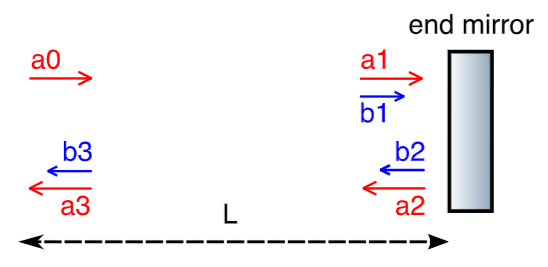
\includegraphics[width=0.4\linewidth]{singlearmmichelson.png}
    \caption{Simplified sketch of a single arm of the Michelson interferometer, the arrows show the carrier fields, denoted by $a$, and the signal sidebands $b$ at the locations where they are computed}
\end{figure}

To determine the response of a Michelson interferometer, the carrier field propagating along each arm must be considered. The forward and return propagation of the carrier are described by
\begin{align}
a_1 = a_0e^{-ik_0L}, \quad
a_2 = r_{\mathrm{ETM}}a_1, \quad
a_3 = a_2e^{-ik_0L},
\end{align}

where \(r_{\mathrm{ETM}}\) is the amplitude reflectivity of the end mirror. During both the forward and return propagation, the carrier acquires the gravitational-wave-induced phase modulation, thereby generating upper and lower signal sidebands in each arm.

The sidebands generated during the forward propagation are
$b_1^{\pm}=a_0\alpha_{\mathrm{gw}}^{\pm},$
which are reflected by the end mirror,
$b_2^{\pm}=r_{\mathrm{etm}}\,b_1^{\pm},$
and propagate back through the arm while accumulating the propagation phase of the sideband frequency,
$b_2^{\pm}e^{-i(k_0\pm k_{\mathrm{gw}})L}$.

During the return trip, the reflected carrier field $a_2$ is itself phase-modulated by the gravitational wave, generating an additional pair of sidebands. Therefore, the total sideband field leaving the arm is
\begin{align}
b_3^{\pm}
&=
b_2^{\pm}e^{-i(k_0\pm k_{\mathrm{gw}})L}
+a_2\alpha_{\mathrm{gw}}^{\pm} \nonumber\\
&=
2r_{\mathrm{etm}}a_0\alpha_{\mathrm{gw}}^{\pm}
e^{-ik_0L}
e^{\mp i k_{\mathrm{gw}}L/2}
\cos\!\left(\frac{k_{\mathrm{gw}}L}{2}\right).
\end{align}

Substituting the sideband amplitude obtained (Eqn. 5.20), and simplifying, the sidebands emerging from the arm become
\begin{equation}
b_3^{\pm}
=
-i\,r_{\mathrm{etm}}a_0
\frac{\omega_0h_0}{2\omega_{\mathrm{gw}}}
\sin(k_{\mathrm{gw}}L)
e^{-i2k_0L}
e^{\pm i(\omega_{\mathrm{gw}}t-k_{\mathrm{gw}}L+\phi_{\mathrm{gw}})}.
\end{equation}

This expression shows that the gravitational-wave signal sidebands are proportional to the strain amplitude $h_0$ and are modulated by the factor $\sin(k_{\mathrm{gw}}L)$, which represents the frequency response of a single interferometer arm. Consequently, the sideband amplitude vanishes whenever
\begin{equation}
k_{\mathrm{gw}}L=N\pi,
\quad
\text{or equivalently,}
\quad
f_{\mathrm{gw}}
=
\frac{Nc}{2L},
\quad N \in \mathbb{N}
\end{equation}

At these frequencies, the phase modulation accumulated during the forward and return trips cancels.

The response of the complete Michelson interferometer is obtained by combining the gravitational-wave sidebands generated in both arms with the carrier field at the output port. Assuming the interferometer operates with a small DC offset from the dark fringe (Section~5.2.1), the output field is
\begin{equation}
E_{\mathrm{out}}
=
i\,2rtE_0\cos(k_0\Delta L)
+b_N^{+}+b_N^{-}+b_E^{+}+b_E^{-},
\end{equation}

where the first term is the leaked carrier acting as the local oscillator, while the remaining terms are the gravitational-wave signal sidebands returning from the North and East arms.

For perfectly reflecting end mirrors ($r_{\mathrm{etm}}=1$), the sidebands generated in each arm follow directly from the single-arm result derived previously. Since the carrier field entering the North arm is $rE_0$ whereas that entering the East arm is $itE_0$, the corresponding sidebands are
\begin{align}
b_N^{\pm}
&=
rtE_0
\frac{\omega_0h_0}{2\omega_{\mathrm{gw}}}
\sin(k_{\mathrm{gw}}L_N)
e^{-i2k_0L_N}
e^{\pm i(\omega_{\mathrm{gw}}t-k_{\mathrm{gw}}L_N+\phi_{\mathrm{gw}})},
\\
b_E^{\pm}
&=
-rtE_0
\frac{\omega_0h_0}{2\omega_{\mathrm{gw}}}
\sin(k_{\mathrm{gw}}L_E)
e^{-i2k_0L_E}
e^{\pm i(\omega_{\mathrm{gw}}t-k_{\mathrm{gw}}L_E+\phi_{\mathrm{gw}})}.
\end{align}

The additional minus sign for the East-arm contribution reflects the differential action of a gravitational wave, which stretches one arm while compressing the other.

To simplify the expressions, the arm lengths are written in terms of their common and differential components, and the following assumptions are made:
\begin{itemize}
\item a $50{:}50$ beam splitter ($r=t=1/\sqrt{2}$),
\item the common arm length is resonant for the carrier,
      $e^{-i2k_0\bar L}=1$,
\item $\bar L\gg\Delta L$,
\item the gravitational-wave wavelength is much larger than the arm-length asymmetry,
      $k_{\mathrm{gw}}(\bar L\pm\Delta L/2)\approx k_{\mathrm{gw}}\bar L$.
\end{itemize}

Under these approximations,
\begin{align}
b_N^{\pm}
&=
E_0
\frac{\omega_0h_0}{4\omega_{\mathrm{gw}}}
\sin(k_{\mathrm{gw}}\bar L)
e^{-ik_0\Delta L}
e^{\pm i(\omega_{\mathrm{gw}}t-k_{\mathrm{gw}}\bar L+\phi_{\mathrm{gw}})},
\\
b_E^{\pm}
&=
-
E_0
\frac{\omega_0h_0}{4\omega_{\mathrm{gw}}}
\sin(k_{\mathrm{gw}}\bar L)
e^{ik_0\Delta L}
e^{\pm i(\omega_{\mathrm{gw}}t-k_{\mathrm{gw}}\bar L+\phi_{\mathrm{gw}})}.
\end{align}

Adding the four sidebands yields
\begin{equation}
b_N^{+}+b_N^{-}+b_E^{+}+b_E^{-}
=
iE_0
\frac{\omega_0h_0}{\omega_{\mathrm{gw}}}
\sin(k_{\mathrm{gw}}\bar L)
\sin(k_0\Delta L)
\cos\!\left(
\omega_{\mathrm{gw}}t-k_{\mathrm{gw}}\bar L+\phi_{\mathrm{gw}}
\right).
\end{equation}

The total field at the antisymmetric port therefore becomes
\begin{equation}
\boxed{
E_{\mathrm{out}}
=
iE_0\cos(k_0\Delta L)
+
iE_0
\frac{\omega_0h_0}{\omega_{\mathrm{gw}}}
\sin(k_{\mathrm{gw}}\bar L)
\sin(k_0\Delta L)
\cos\!\left(
\omega_{\mathrm{gw}}t-k_{\mathrm{gw}}\bar L+\phi_{\mathrm{gw}}
\right)}.
\end{equation}

The photodiode measures the optical power, $P_{\mathrm{out}}=|E_{\mathrm{out}}|^2$. Retaining only the terms linear in the gravitational-wave strain gives
\begin{equation}
P_{\mathrm{gw}}
=
|E_0|^2
\frac{\omega_0h_0}{\omega_{\mathrm{gw}}}
\sin(k_{\mathrm{gw}}\bar L)
\sin(2k_0\Delta L)
\cos\!\left(
\omega_{\mathrm{gw}}t-k_{\mathrm{gw}}\bar L+\phi_{\mathrm{gw}}
\right).
\end{equation}

For DC readout, the interferometer is operated slightly away from the dark fringe,$
\Delta L=\frac{\pi}{2k_0}+\delta_{\mathrm{off}},\
\delta_{\mathrm{off}}\ll\lambda_0.
$ Using the small-angle approximation,
$\sin(2k_0\Delta L)
\simeq
2k_0\delta_{\mathrm{off}}$, the detected gravitational-wave signal simplifies to
\begin{equation}
P_{\mathrm{gw}}
\approx
2k_0\delta_{\mathrm{off}}
|E_0|^2
\frac{\omega_0h_0}{\omega_{\mathrm{gw}}}
\sin(k_{\mathrm{gw}}\bar L)
\cos\!\left(
\omega_{\mathrm{gw}}t-k_{\mathrm{gw}}\bar L+\phi_{\mathrm{gw}}
\right).
\end{equation}

This expression clearly shows that a finite DC offset is essential for detection. The leaked carrier provides the local oscillator that beats with the gravitational-wave sidebands, converting the optical phase modulation into a measurable intensity modulation at the photodetector.

Finally, the transfer function from the gravitational-wave strain to the detected optical power is
\begin{equation}
T_{\mathrm{gw}\rightarrow P}(\omega_{\mathrm{gw}})
\approx
k_0\delta_{\mathrm{off}}
|E_0|^2
\frac{\omega_0}{\omega_{\mathrm{gw}}}
\sin(k_{\mathrm{gw}}\bar L)
e^{-ik_{\mathrm{gw}}\bar L},
\end{equation}

which describes the frequency-dependent response of a DC-readout Michelson interferometer to an incident gravitational wave.







\chapter{Beyond the Plane-Wave Approximation}

The plane wave model provides a simple and powerful framework for understanding many fundamental aspects of interferometry. Using this approximation, optical fields can be described entirely through their amplitudes and phases, allowing straightforward analysis of propagation, reflection, transmission, modulation, and cavity resonance. Consequently, the plane wave model forms the foundation of many analytical treatments of interferometric systems.

However, real laser beams are not plane waves. A plane wave is assumed to have an infinite transverse extent and uniform intensity across all space, making it an idealised mathematical construct rather than a physically realisable optical field. In practice, laser beams possess finite transverse dimensions and exhibit spatially varying intensity and phase distributions.

For precision interferometric applications, particularly gravitational wave detectors, these spatial effects play a crucial role in determining optical performance and sensitivity. The propagation of realistic laser beams must therefore be treated using solutions of the wave equation that account for the electromagnetic field's transverse structure.

\section{The Paraxial Approximation}

To describe realistic laser beams, we must move beyond the plane wave approximation and consider the full electromagnetic wave equation. In free space, each component of the electric field satisfies the homogeneous wave equation

\begin{equation}
\nabla^2 E - \frac{1}{c^2}\frac{\partial^2 E}{\partial t^2}=0.
\end{equation}

For monochromatic light, the electric field can be written as

\begin{equation}
E(\mathbf{r},t)=U(\mathbf{r})e^{i\omega t},
\end{equation}

where $U(\mathbf{r})$ contains the spatial dependence of the field and $\omega$ is the angular frequency. Substituting this expression into the wave equation yields

\begin{equation}
\nabla^2 U + k^2 U = 0,
\end{equation}

This equation is known as the \textit{\textbf{Helmholtz equation}} and governs the spatial behaviour of monochromatic optical fields.

To obtain solutions describing laser beams propagating primarily along the $z$-axis, the field is written as

\begin{equation}
U(x,y,z)=u(x,y,z)e^{-ikz},
\end{equation}

where the rapidly oscillating phase factor $e^{-ikz}$ represents the dominant propagation and the function $u(x,y,z)$ varies slowly along the propagation direction.

Substituting this form into the Helmholtz equation gives

\begin{equation}
\frac{\partial^2 u}{\partial x^2}
+
\frac{\partial^2 u}{\partial y^2}
+
\frac{\partial^2 u}{\partial z^2}
-
2ik\frac{\partial u}{\partial z}
=
0.
\end{equation}

For laser beams whose transverse extent changes only gradually along the propagation direction, the envelope function $u$ varies slowly with $z$. Under this condition,

\begin{equation}
\left|
\frac{\partial^2 u}{\partial z^2}
\right|
\ll
\left|
2ik\frac{\partial u}{\partial z}
\right|,
\end{equation}

allowing the second-order longitudinal derivative to be neglected. This approximation is known as the \textit{paraxial approximation}.

The resulting equation,

\begin{equation}
\boxed{\frac{\partial^2 u}{\partial x^2}
+
\frac{\partial^2 u}{\partial y^2}
-
2ik\frac{\partial u}{\partial z}
=
0}
\end{equation}

is called the \textit{\textbf{paraxial wave equation}}. Its solutions describe realistic laser beams with finite transverse extent and form the basis of Gaussian beam optics. In the following sections, we derive the Gaussian beam solution and examine its fundamental properties.

\section{Hermite-Gaussian Modes}

The paraxial wave equation admits an infinite number of solutions describing optical fields with finite transverse extent. While the fundamental Gaussian beam is the simplest such solution, a complete description of realistic laser beams often requires a broader set of solutions known as the \textit{Hermite--Gaussian (HG) modes}. These modes form a complete, countable set of orthonormal solutions to the paraxial wave equation and are commonly referred to as transverse electromagnetic (TEM) modes.

The importance of Hermite-Gaussian modes lies in their completeness. Any solution of the paraxial wave equation can be expressed as a linear combination of these modes. If $u'(x,y,z)$ represents an arbitrary paraxial optical field, then it may be written as
\begin{equation}
u'(x,y,z)
=
\sum_{n,m}
a_{nm}\,u_{nm}(x,y,z),
\end{equation}

where $u_{nm}(x,y,z)$ denotes the Hermite--Gaussian mode of order $(n,m)$ and $a_{nm}$ are the corresponding expansion coefficients.

Consequently, any beam-like electromagnetic field can be represented as a superposition of Hermite-Gaussian modes,
\begin{equation}
E(t,x,y,z)
=
\sum_j
\sum_{n,m}
a_{jnm}
u_{nm}(x,y,z)
e^{i(\omega_j t-k_j z)}.
\end{equation}

The indices $n$ and $m$ specify the transverse mode order in the horizontal and vertical directions, respectively. The lowest-order mode, $\mathrm{TEM}_{00}$, corresponds to the fundamental Gaussian beam, while higher-order modes exhibit increasingly complex transverse intensity distributions.

A particularly useful property of Hermite-Gaussian modes is their orthonormality. They satisfy
\begin{equation}
\iint
u_{nm}
u_{n'm'}^{*}
\,dx\,dy
=
\delta_{nn'}
\delta_{mm'},
\end{equation}

where $\delta$ denotes the Kronecker delta. This orthogonality implies that different modes are mutually independent and can be treated as basis vectors in the function space of paraxial optical fields.

The orthonormal nature of the Hermite--Gaussian modes also simplifies power calculations. For a beam expanded in this basis, the total optical power is simply the sum of the powers contained in each mode:
\begin{equation}
P
=
EE^{*}
=
\sum_{n,m}
a_{nm}a_{nm}^{*}.
\end{equation}

For optical fields containing multiple frequency components, the detected power becomes
\begin{equation}
P
=
EE^{*}
=
\sum_{n,m}
\sum_i
\sum_j
a_{inm}a_{jnm}^{*},
\qquad
\omega_i=\omega_j.
\end{equation}

The complete set of Hermite-Gaussian modes consists of an infinite discrete family of functions $u_{nm}(x,y,z)$, where the integers $n$ and $m$ denote the mode numbers in the horizontal and vertical directions, respectively. The quantity $N = n+m$ is known as the \textit{mode order}. Modes with $N>0$ are generally referred to as higher-order modes, while the $\mathrm{TEM}_{00}$ mode corresponds to the fundamental Gaussian beam.

The Hermite-Gaussian modes can be written as the product of two one-dimensional solutions,
\begin{equation}
u_{nm}(x,y,z)
=
u_n(x,z)\,u_m(y,z),
\end{equation}
where
\begin{equation}
u_n(x,z)
=
\left(
\frac{\sqrt{2/\pi}}
     {2^n n! \, w(z)}
\right)^{1/2}
H_n\!\left(
\frac{\sqrt{2}x}{w(z)}
\right)
\exp\!\left[
-\frac{x^2}{w^2(z)}
-\frac{ikx^2}{2R_C(z)}
+i(2n+1)\Psi(z)
\right].
\end{equation}

Here, $H_n(x)$ denotes the Hermite polynomial of order $n$, $w(z)$ is the beam radius, $R_C(z)$ is the radius of curvature of the wavefront, and $\Psi(z)$ is the Gouy phase.

The first few Hermite polynomials are
\begin{align}
H_0(x) &= 1, \\
H_1(x) &= 2x, \\
H_2(x) &= 4x^2-2, \\
H_3(x) &= 8x^3-12x.
\end{align}

Higher-order polynomials may be generated recursively using
\begin{equation}
H_{n+1}(x)
=
2xH_n(x)
-
2nH_{n-1}(x).
\end{equation}

Combining the horizontal and vertical solutions yields the two-dimensional Hermite--Gaussian mode
\begin{align}
u_{nm}(x,y,z)
&=
\left(
\frac{2^{\,1-n-m}}
     {\pi\,n!\,m!}
\right)^{1/2}
\frac{1}{w(z)}
\exp\!\left[i(n+m+1)\Psi(z)\right]
\nonumber\\
&\quad\times
H_n\!\left(\frac{\sqrt{2}x}{w(z)}\right)
H_m\!\left(\frac{\sqrt{2}y}{w(z)}\right)
\exp\!\left[
-\frac{x^2+y^2}{w^2(z)}
-\frac{ik(x^2+y^2)}{2R_C(z)}
\right].
\end{align}

This expression explicitly reveals the additional longitudinal phase factor $(n+m+1)\Psi(z)$, known as the \textit{Gouy phase}. Unlike a plane wave, each Hermite--Gaussian mode accumulates an extra phase shift during propagation, with higher-order modes acquiring proportionally larger Gouy phase shifts. 

\section{Properties of Higher-Order Hermite--Gaussian Modes}
\begin{enumerate}
    \item \textbf{Transverse Structure:}  
    The mode indices $n$ and $m$ determine the number of nodes in the horizontal and vertical directions, respectively. As a result, higher-order modes exhibit increasingly complex intensity distributions with multiple lobes separated by nodal lines.

    \item \textbf{Symmetry:}  
    Owing to the separable form $u_{nm}(x,y,z)=u_n(x,z)u_m(y,z)$,
    the transverse intensity pattern exhibits a natural symmetry between the $x$ and $y$ directions.

    \item \textbf{Increasing Beam Size:}  
    For a fixed optical power, the spatial extent of the intensity distribution increases with mode order. Consequently, higher-order modes occupy a larger area while exhibiting a lower peak intensity.

    \item \textbf{Shape Preservation During Propagation:}  
    The transverse shape of a Hermite--Gaussian mode remains unchanged during propagation. While the beam size scales according to Gaussian beam propagation, the overall intensity pattern is preserved.

    \item \textbf{Common Wavefront Curvature:}  
    All Hermite--Gaussian modes associated with the same Gaussian beam parameter share the same radius of curvature $R_C(z)$. The curvature evolves with propagation but is independent of the mode order.

    \item \textbf{Mode-Dependent Gouy Phase:}  
    Higher-order modes acquire an additional longitudinal phase shift given by $\phi=(n+m+1)\Psi(z)$. Thus, higher-order modes accumulate larger Gouy phase shifts than the fundamental mode.

    \item \textbf{Orthogonality:}  
    Hermite--Gaussian modes are orthonormal and satisfy
    $
    \iint u_{nm}u_{n'm'}^{*}\,dx\,dy
    =
    \delta_{nn'}\delta_{mm'}.
    $    This property allows arbitrary paraxial fields to be expanded uniquely in terms of Hermite--Gaussian modes.

    \item \textbf{Completeness:}  
    The Hermite--Gaussian modes form a complete basis for solutions of the paraxial wave equation, enabling any physically realizable paraxial beam to be represented as a superposition of these modes.
\end{enumerate}

\section{Gaussian Beam Optics}

The fundamental solution of the paraxial wave equation is the lowest-order Hermite--Gaussian mode, commonly referred to as the \textit{Gaussian beam} ($TEM_{00}$). Unlike a plane wave, which extends infinitely in the transverse directions, a Gaussian beam possesses a finite spatial extent and therefore provides a much more realistic description of laser light. Most practical laser beams operate predominantly in this fundamental mode, making Gaussian beam optics the foundation of modern interferometry.

The electric field distribution of a Gaussian beam is given by
\begin{equation}
\boxed{
u(x,y,z)
=
\sqrt{\frac{2}{\pi}}
\frac{1}{w(z)}
\exp\!\left(i\Psi(z)\right)
\exp\!\left[
-\frac{ik(x^2+y^2)}{2R_C(z)}
-\frac{x^2+y^2}{w^2(z)}
\right]}
\end{equation}

Several parameters appear in this expression that describe the beam's evolution during propagation. These include the beam radius $w(z)$, the radius of curvature of the wavefront $R_C(z)$, and the Gouy phase $\Psi(z)$. Together, these quantities completely determine the spatial properties of the beam.

The intensity profile of a Gaussian beam follows a Gaussian distribution in the transverse direction. For a beam carrying total power $P$, the radial intensity distribution is
\begin{equation}
I(r)
=
\frac{2P}{\pi w^2(z)}
\exp\!\left(
-\frac{2r^2}{w^2(z)}
\right),
\end{equation}
where $r^2=x^2+y^2$. The parameter $w(z)$ is known as the beam radius or spot size and is defined as the radius at which the intensity falls to $1/e^2$ of its peak value.

\begin{figure}[!ht]
    \centering
    \includegraphics[width=\linewidth]{wz.png}
    \caption{typical laser beam intensity pattern (left) and the intensity and amplitude distributions of a normalised Gaussian beam (right). A Gaussian beam is characterised by its spot size, w, the radius at which the intensity falls to $1/e^2$ ($\sim14 \%$) of the peak intensity}
\end{figure}

A Gaussian beam is completely specified by two parameters: the minimum beam radius $w_0$, called the \textit{beam waist}, and the waist position $z_0$ along the propagation axis. From these quantities, several useful beam parameters can be derived.

\subsection{Rayleigh Range and Beam Size}
A Gaussian beam can be divided into two distinct propagation regions: the near field, located around the beam waist, and the far field, where diffraction dominates the beam evolution. The characteristic length scale separating these regions is known as the \textit{Rayleigh range}, denoted by $z_R$.

The Rayleigh range is related to the beam waist $w_0$ and the wavelength $\lambda$ by
\begin{equation}
z_R = \frac{\pi w_0^2}{\lambda}.
\end{equation}

Using the Rayleigh range, the beam radius at any position $z$ can be written as
\begin{equation}
w(z)
=
w_0
\sqrt{
1+
\left(
\frac{z-z_0}{z_R}
\right)^2
},
\end{equation}
where $z_0$ is the location of the beam waist.

This expression shows that the beam radius reaches its minimum value $w_0$ at the waist and increases symmetrically on either side due to diffraction. The Rayleigh range corresponds to the distance from the waist at which the beam area has doubled, or equivalently where $w(z_R)=\sqrt{2}\,w_0$.

Far from the waist, where $|z-z_0| \gg z_R$, the beam radius grows approximately linearly with distance:
\begin{equation}
w(z)
\approx
w_0\frac{|z-z_0|}{z_R}
=
\frac{\lambda |z-z_0|}{\pi w_0}.
\end{equation}

This linear expansion is a direct consequence of diffraction and characterises the far-field behaviour of the beam.

\begin{figure}[!ht]
    \centering
    \includegraphics[width=0.9\linewidth]{gaussbeamcrosssec.png}
    \caption{Gaussian beam profile along $z$: this cross section along the x–z plane illustrates how the beam size $w(z)$ of the Gaussian beam changes along the optical axis. The position of minimum beam size $w_0$ is called beam waist.}
\end{figure}

\subsection{Diffraction Angle}

The divergence of a Gaussian beam in the far field is quantified by the diffraction angle $\Theta$. This angle is defined as the asymptotic angle between the beam envelope and the optical axis.

Using the far-field approximation for the beam radius, the diffraction angle is given by
\begin{equation}
\Theta
=
\arctan\left(
\frac{w_0}{z_R}
\right)
=
\arctan\left(
\frac{\lambda}{\pi w_0}
\right).
\end{equation}

For most laser beams, the diffraction angle is small and therefore
\begin{equation}
\Theta
\approx
\frac{\lambda}{\pi w_0}.
\end{equation}

This relation illustrates an important trade-off in Gaussian beam optics: larger beam waists produce smaller diffraction angles and therefore less beam spreading during propagation.

\subsection{Radius of Curvature}

As a Gaussian beam propagates, its phase fronts are generally curved rather than planar. The curvature of these phase fronts is described by the radius of curvature $R_C(z)$.

The radius of curvature as a function of propagation distance is
\begin{equation}
R_C(z)
=
(z-z_0)
+
\frac{z_R^2}{z-z_0}.
\end{equation}

Several important limits can be identified:
\begin{align}
R_C(z) &\rightarrow \infty,
\qquad |z-z_0| \ll z_R, \\
R_C(z) &\approx z-z_0,
\qquad |z-z_0| \gg z_R, \\
R_C(z) &= 2z_R,
\qquad z-z_0=z_R.
\end{align}

At the beam waist, the phase fronts are locally planar and the radius of curvature becomes infinite. As the beam propagates away from the waist, the phase fronts become increasingly curved. In the far field, the radius of curvature approaches the propagation distance itself, corresponding to a spherical wavefront centred at the beam waist.44

\subsection{The Gaussian Beam Parameter}
A particularly convenient way of describing Gaussian beams is through the \textit{Gaussian beam parameter}, commonly denoted by $q$. This complex parameter combines both the beam size and the wavefront curvature into a single quantity, greatly simplifying the analysis of beam propagation through optical systems.

The Gaussian beam parameter is defined as
\begin{equation}
\frac{1}{q(z)}
=
\frac{1}{R_C(z)}
-
i\frac{\lambda}{\pi w^2(z)},
\end{equation}
where $R_C(z)$ is the radius of curvature of the wavefront and $w(z)$ is the beam radius.

Using the definitions of the beam waist and Rayleigh range, the beam parameter may also be written as
\begin{equation}
\boxed{
q(z)
=
(z-z_0)+iz_R},
\end{equation}

or equivalently, $q(z)=q_0+(z-z_0)$, where $q_0 = iz_R$ is the beam parameter at the waist. Expressed in terms of the $q$-parameter, the fundamental Gaussian beam takes the compact form \footnote{The Gaussian beam parameter can also be used to express the Hermite--Gaussian modes in a more compact form. Using the complex beam parameter $q(z)$, the modes can be written as $u_{nm}(x,y,z)=u_n(x,z)\,u_m(y,z)$, where
\begin{align}
u_n(x,z)
&=
\left(\frac{2}{\pi}\right)^{1/4}
\left(\frac{1}{2^n n! \, w_0}\right)^{1/2}
\left(\frac{q_0}{q(z)}\right)^{1/2}
\left(
\frac{q_0 q^*(z)}
     {q_0^* q(z)}
\right)^{n/2}
H_n\!\left(
\frac{\sqrt{2}x}{w(z)}
\right)
\exp\!\left(
-\frac{ikx^2}{2q(z)}
\right).
\end{align}}
\begin{equation}
\boxed{
u(x,y,z)
=
\sqrt{\frac{2}{\pi}}
\frac{q_0}{w_0\,q(z)}
\exp\!\left[
-\frac{ik(x^2+y^2)}{2q(z)}
\right]}
\end{equation}

The principal beam properties can also be obtained directly from the beam parameter. 
\begin{table}[h]
\centering
\caption{Gaussian beam quantities expressed using the beam parameter $q$.}
\begin{tabular}{c|c|c|c}

$\displaystyle w^2(z)=\frac{\lambda}{\pi}\frac{|q|^2}{\Im\{q\}}$
&
$\displaystyle w_0^2=\frac{\lambda}{\pi}\Im\{q\}$
&
$\displaystyle z_R=\Im\{q\}$
&
$\displaystyle R_C(z)=\frac{|q|^2}{\Re\{q\}}$
\\

\end{tabular}
\label{tab:q_parameter_summary}
\end{table}

The Gaussian beam parameter therefore provides a compact and powerful description of Gaussian beam propagation. Its greatest utility arises when analysing optical systems using matrix methods, where the evolution of a beam through lenses, mirrors, and free space can be expressed through simple transformations of the $q$-parameter.

\section{Gouy Phase}

An important feature of Gaussian and Hermite--Gaussian beams is the presence of an additional longitudinal phase shift known as the \textit{Gouy phase}. Unlike a plane wave, which accumulates phase linearly during propagation, a Gaussian beam experiences an extra phase lag as it passes through its focal region. Physically, this effect reflects the slightly reduced phase velocity of confined optical beams compared to ideal plane waves.

For a Gaussian beam, the Gouy phase is given by
\begin{equation}
\Psi(z)
=
\arctan\left(
\frac{z-z_0}{z_R}
\right),
\end{equation}
where $z_0$ is the beam waist location and $z_R$ is the Rayleigh range.

Using the Gaussian beam parameter, the same quantity can be written as
\begin{equation}
\Psi(z)
=
\arctan\left(
\frac{\Re\{q\}}
     {\Im\{q\}}
\right).
\end{equation}

The Gouy phase contributes an additional phase shift to Hermite--Gaussian modes. Relative to a plane wave, the total phase lag is
\begin{equation}
\phi
=
(n+m+1)\Psi(z),
\end{equation}
where $n$ and $m$ are the transverse mode indices.

As a consequence, higher-order modes accumulate larger phase shifts during propagation. This additional phase plays an important role in optical resonators, where it modifies the resonance conditions of different transverse modes and determines the spacing between cavity eigenfrequencies.

\section{Simulating of Hermite-Gaussian Mode Transverse Intensity Profiles}

\begin{lstlisting}[language=Python]
import numpy as np
import matplotlib.pyplot as plt
from scipy.special import hermite

def hermite_gauss_mode(x, y, m, n, w0):
    """Calculate the Hermite-Gauss mode field distribution."""
    Hm = hermite(m)(np.sqrt(2) * x / w0)
    Hn = hermite(n)(np.sqrt(2) * y / w0)
    return Hm * Hn * np.exp(-(x**2 + y**2) / w0**2)

# Parameters
w0 = 1.0  # Beam waist
x = np.linspace(-3*w0, 3*w0, 100)
y = np.linspace(-3*w0, 3*w0, 100)
X, Y = np.meshgrid(x, y)

fig, axes = plt.subplots(4, 4, figsize=(12, 12))
modes = [(0, 0), (1, 0), (2, 0), (3, 0),
         (0, 1), (1, 1), (2, 1), (3, 1),
         (0, 2), (1, 2), (2, 2), (3, 2),
         (0, 3), (1, 3), (2, 3), (3, 3)]

for ax, (m, n) in zip(axes.flatten(), modes):
    field = hermite_gauss_mode(X, Y, m, n, w0)
    ax.contourf(X, Y, field, levels=50, cmap='viridis')
    ax.set_title(f'm={m}, n={n}')
    ax.set_xlabel('x')
    ax.set_ylabel('y')
    ax.axis('equal')
plt.tight_layout()
plt.show()
\end{lstlisting}

\begin{figure}[!ht]
    \centering
    \includegraphics[width=\linewidth]{hgmodes.png}
    \caption{Transverse intensity distributions of Hermite-Gaussian modes $TEM_{00}$ tp $TEM_{33}$}
\end{figure}

\section{Laguerre-Gaussian Modes}

Laguerre-Gaussian (LG) modes constitute another complete set of solutions to the paraxial wave equation. Unlike Hermite--Gaussian modes, which are naturally expressed in Cartesian coordinates, Laguerre--Gaussian modes are defined in cylindrical coordinates and are therefore particularly well suited to optical systems possessing cylindrical symmetry.

Interest in Laguerre-Gaussian modes extends beyond mathematical convenience. In the context of gravitational-wave detectors, higher-order Laguerre-Gaussian beams have been proposed as alternatives to the fundamental Gaussian mode because their broader intensity distributions can reduce the impact of mirror thermal noise, thereby improving detector sensitivity.

The general form of a helical Laguerre--Gaussian mode is
\begin{align}
u_{p,l}(r,\phi,z)=
\frac{1}{w(z)}
\sqrt{\frac{2\,p!}{\pi (|l|+p)!}}
\exp\!\left[i(2p+|l|+1)\Psi(z)\right]
\left(
\frac{\sqrt{2}r}{w(z)}
\right)^{|l|}
L_p^{|l|}
\!\left(
\frac{2r^2}{w^2(z)}
\right)
\exp\!\left(
-\frac{ikr^2}{2q(z)}
+i l\phi
\right),
\end{align}
where $r$, $\phi$, and $z$ are cylindrical coordinates, $p$ is the radial mode index, $l$ is the azimuthal mode index, and $L_p^{|l|}(x)$ denotes the associated Laguerre polynomial.

The associated Laguerre polynomials are defined by
\begin{equation}
L_p^{|l|}(x)
=
\frac{1}{p!}
\sum_{j=0}^{p}
\frac{p!}{j!}
\binom{|l|+p}{p-j}
(-x)^j.
\end{equation}

All other beam parameters, including the beam radius $w(z)$, beam parameter $q(z)$, Rayleigh range, and Gouy phase, retain the same definitions as for Hermite--Gaussian modes.

\subsection{Sinusoidal Laguerre--Gaussian Modes}

The helical Laguerre--Gaussian modes described above possess a spiral phase front arising from the azimuthal phase factor $e^{il\phi}$. While this representation is mathematically elegant and directly exhibits the orbital angular momentum of the beam, an alternative form of Laguerre--Gaussian modes is often encountered in optical resonator studies and interferometric simulations.

These modes are obtained by replacing the azimuthal phase factor with a sinusoidal angular dependence, typically $\cos(l\phi)$ or $\sin(l\phi)$. The resulting field distribution may be written as
\begin{align}
u^{\mathrm{alt}}_{p,l}(r,\phi,z)
&=
\frac{2}{w(z)}
\sqrt{
\frac{p!}
     {(1+\delta_{0l})\pi(|l|+p)!}
}
\exp\!\left[i(2p+|l|+1)\Psi(z)\right]
\nonumber\\
&\quad\times
\left(
\frac{\sqrt{2}r}{w(z)}
\right)^{|l|}
L_p^{|l|}
\!\left(
\frac{2r^2}{w^2(z)}
\right)
\exp\!\left(
-\frac{ikr^2}{2q(z)}
\right)
\cos(l\phi).
\end{align}

Unlike helical Laguerre--Gaussian modes, sinusoidal Laguerre-Gaussian modes do not possess a spiral phase structure. Instead, their phase fronts remain spherical, similar to those of Hermite-Gaussian modes. The azimuthal dependence appears directly in the amplitude distribution, producing characteristic dark radial lines in addition to the concentric rings determined by the radial index $p$.

This distinction leads to markedly different transverse intensity patterns. Helical Laguerre-Gaussian modes exhibit rotationally symmetric ring-shaped intensity distributions, whereas sinusoidal Laguerre--Gaussian modes display angular nodal lines that divide the beam into multiple lobes. The number of these nodal lines increases with the azimuthal mode index $l$.

From a practical perspective, sinusoidal Laguerre--Gaussian modes are often more convenient for optical cavity simulations because they possess real-valued transverse mode structures and can be treated analogously to Hermite--Gaussian modes. In contrast, helical Laguerre-Gaussian modes are particularly useful when studying orbital angular momentum and vortex beam phenomena, where the spiral phase structure plays a central role.

Both the helical and sinusoidal Laguerre-Gaussian modes form complete sets of solutions to the paraxial wave equation and can therefore be used as basis functions for describing arbitrary paraxial optical fields.

\subsection{Physical Characteristics}

A defining feature of Laguerre-Gaussian modes is their azimuthal phase dependence through the factor $e^{il\phi}$. This term gives rise to a helical phase structure in which the phase winds around the beam axis. As a consequence, the wavefront forms a spiral rather than a plane or spherical surface.

The intensity distribution of Laguerre-Gaussian modes is markedly different from that of Hermite-Gaussian modes. Instead of rectangular patterns with nodal lines, Laguerre-Gaussian modes exhibit concentric ring structures centred on the optical axis. The number of rings is determined primarily by the radial index $p$, while the azimuthal index $l$ governs the phase winding around the beam.

Because of their helical phase structure, Laguerre-Gaussian modes carry orbital angular momentum. Each photon in an $\mathrm{LG}_{p,l}$ mode carries an orbital angular momentum of $l\hbar$, making these modes important in applications ranging from optical manipulation and quantum optics to advanced interferometric sensing.

\section{Simulating helical Laguerre-Gaussian Mode Transverse In-
tensity Profiles}

\begin{lstlisting}[language=Python]
import numpy as np
import matplotlib.pyplot as plt
from scipy.special import genlaguerre, factorial

def laguerre_gauss(p, l, X, Y, w0=1.0):
    """
    Helical Laguerre-Gauss mode LG(p,l) at z = 0.

    Parameters
    p (int) : Radial index (p >= 0)
    l (int) : Azimuthal index
    X, Y (ndarray) : Meshgrid coordinates
    w0 (float) : Beam waist

    Returns
    U (complex ndarray): Complex field amplitude
    """

    r = np.sqrt(X**2 + Y**2)
    phi = np.arctan2(Y, X)
    rho = 2 * r**2 / w0**2
    L = genlaguerre(p, abs(l))(rho)
    norm = np.sqrt(2 * factorial(p) / (np.pi * factorial(p + abs(l))))
    U = (norm * (np.sqrt(2) * r / w0)**abs(l) * L * np.exp(-r**2 / w0**2) * np.exp(1j * l * phi))

    return U

fig, axes = plt.subplots(4, 4, figsize=(12, 12))
modes = [(0,0), (0,1), (0,2), (0,3),
        (1,0), (1,1), (1,2), (1,3),
        (2,0), (2,1), (2,2), (2,3),
        (3,0), (3,1), (3,2), (3,3)]

for ax, (p, l) in zip(axes.flatten(), modes):
    E = laguerre_gauss_mode(X, Y, p, l, w0)
    I = np.abs(E)**2

    ax.contourf(X, Y, I, levels=50, cmap='inferno')
    ax.set_title(f'LG({p},{l})')
    ax.set_aspect('equal')

plt.tight_layout()
plt.show()
\end{lstlisting}

\begin{figure}[!ht]
    \centering
    \includegraphics[width=\linewidth]{helicalLGmode.png}
    \caption{Intensity profiles for helical Laguerre–Gauss modes $u_{pl}$ . The $LG_{00}$ mode is identical to the Hermite–Gauss mode of order 0. Higher-order modes show a widening of the intensity and decreasing peak intensity. The number of concentric dark rings is given by the radial mode index $p$}
\end{figure}

\section{Simulating sinusoidal Laguerre-Gaussian Mode Transverse Intensity Profiles}

\begin{lstlisting}[language=Python]
def sinusoidal_laguerre_gauss(p, l, X, Y, w0=1.0):
    """
    Parameters
    p (int) : Radial index (p >= 0)
    l (int) : Azimuthal index
    X, Y (ndarray) : Meshgrid coordinates
    w0 (float) : Beam waist

    Returns
    U (complex ndarray): Complex field amplitude
    """

    r = np.sqrt(X**2 + Y**2)
    phi = np.arctan2(Y, X)
    rho = 2 * r**2 / w0**2
    L = genlaguerre(p, abs(l))(rho)
    norm = np.sqrt(2 * factorial(p) / (np.pi * factorial(p + abs(l))))
    U = (norm * (np.sqrt(2) * r / w0)**abs(l) * L * np.exp(-r**2 / w0**2) * np.cos(l * phi))

    return U

fig, axes = plt.subplots(4, 4, figsize=(12, 12))
modes = [(p, l) for p in range(4) for l in range(4)]
x = np.linspace(-5, 5, 400)
y = np.linspace(-5, 5, 400)
X, Y = np.meshgrid(x, y)
for ax, (p, l) in zip(axes.flatten(), modes):
    U = sinusoidal_laguerre_gauss(p, l, X, Y)
    intensity = np.abs(U)**2
    ax.imshow(intensity, extent=(-5, 5, -5, 5), cmap='inferno')
    ax.set_title(f'LG({p},{l})')
    ax.axis('off')
    
plt.tight_layout()
plt.show()
\end{lstlisting}

\begin{figure}[!ht]
    \centering
    \includegraphics[width=\linewidth]{sinLGmodes.png}
    \caption{ntensity profiles for sinusoidal Laguerre–Gauss modes $u^{alt}_{pl}$ . The $u_{p0}$ modes are identical to the helical modes. However, for azimuthal mode indices $l > 0$ the pattern shows $l$ dark radial lines in addition to the $p$ dark concentric rings}
\end{figure}

\section{Astigmatism}

In the discussions so far, Gaussian, Hermite--Gaussian, and Laguerre--Gaussian beams have been assumed to possess rotational symmetry about the optical axis. In practice, however, many optical systems exhibit \textit{astigmatism}, where the beam properties in two orthogonal transverse planes differ. As a result, the beam can no longer be described by a single beam parameter, spot size, or radius of curvature.

Astigmatism commonly arises from optical elements that possess different curvatures in different directions, such as cylindrical lenses, tilted spherical mirrors, or off-axis reflections from curved surfaces. In gravitational-wave interferometers and optical resonators, astigmatism is frequently encountered due to non-normal incidence on cavity mirrors and beam splitters.

For an astigmatic beam, the tangential and sagittal planes must be treated independently. The beam is therefore described by two separate Gaussian beam parameters,
\begin{equation}
q_t(z)=(z-z_{0,t})+iz_{R,t}, \quad \text{and} \quad
q_s(z)=(z-z_{0,s})+iz_{R,s},
\end{equation}

corresponding to the tangential and sagittal directions, respectively. Consequently, the beam radii and radii of curvature become
\begin{equation}
w_t(z)\neq w_s(z),
\quad
and
\quad
R_t(z)\neq R_s(z).
\end{equation}

The most visible consequence of astigmatism is that the beam cross-section becomes elliptical rather than circular. Furthermore, the beam generally possesses different waist locations in the two transverse directions, resulting in distinct focal positions along the propagation axis.

Astigmatism also affects the Gouy phase. Since the tangential and sagittal beam parameters evolve independently, the Gouy phase must be evaluated separately in each plane:
\begin{equation}
\Psi_t(z)
=
\arctan
\left(
\frac{\Re\{q_t\}}
     {\Im\{q_t\}}
\right),
\quad
and
\quad
\Psi_s(z)
=
\arctan
\left(
\frac{\Re\{q_s\}}
     {\Im\{q_s\}}
\right).
\end{equation}

The total Gouy phase accumulated by a higher-order mode is therefore
\begin{equation}
\phi
=
\left(n+\frac{1}{2}\right)\Psi_t(z)
+
\left(m+\frac{1}{2}\right)\Psi_s(z),
\end{equation}
where $n$ and $m$ are the transverse mode indices.

\section{Ray-Transfer Matrices or ABCD Matrices}
The propagation of Gaussian beams through optical systems can be described efficiently using the formalism of ray transfer matrices, also known as the \textit{ABCD matrix method}. This approach provides a compact mathematical framework for analysing the behaviour of optical rays and Gaussian beams as they propagate through free space and interact with optical components such as lenses, mirrors, and dielectric interfaces.

In geometrical optics, a paraxial ray at a given position along the optical axis can be represented by a two-component vector,
\begin{equation}
\mathbf{r}
=
\begin{pmatrix}
y \\
\theta
\end{pmatrix},
\end{equation}

where $x$ denotes the transverse displacement of the ray from the optical axis and $\theta$ is the angle the ray makes with the optical axis. Under the paraxial approximation, where $\theta \ll 1$, the evolution of the ray through an optical element can be represented by a linear transformation,
\begin{equation}
\begin{pmatrix}
y_2 \\
\theta_2
\end{pmatrix}
=
\begin{pmatrix}
A & B \\
C & D
\end{pmatrix}
\begin{pmatrix}
y_1 \\
\theta_1
\end{pmatrix},
\end{equation}
where the matrix
\begin{equation}
M=
\begin{pmatrix}
A & B \\
C & D
\end{pmatrix}
\end{equation}
is known as the ray transfer matrix of the optical system.

One of the major advantages of this formalism is that complex optical systems can be analysed by simply "\textit{cascading}" the matrices corresponding to individual optical components. If an optical system consists of several elements arranged sequentially, the overall transfer matrix is obtained from
\begin{equation}
M_{\mathrm{total}}
=
M_N M_{N-1}\cdots M_2 M_1.
\end{equation}

The ABCD matrix formalism is particularly important in Gaussian beam optics because the same matrices that describe ray propagation can also be used to determine the evolution of the Gaussian beam parameter. If a beam with parameter $q_1$ propagates from a medium of refractive index $n_1$ into an optical system and emerges with beam parameter $q_2$ in a medium of refractive index $n_2$, then the Gaussian beam parameters are related by
\begin{equation}
\frac{q_2}{n_2}
=
\frac{
A\left(\dfrac{q_1}{n_1}\right)+B
}{
C\left(\dfrac{q_1}{n_1}\right)+D
}.
\end{equation}

\begin{figure}[!ht]
    \centering
    \includegraphics[width=\linewidth]{ABCD.png}
\end{figure}

\section{Cavity Eigenmodes and Stability}
An optical cavity supports only specific field distributions that reproduce themselves after every round-trip inside the resonator. Such self-consistent field distributions are known as \textit{cavity eigenmodes}. For resonators composed of spherical mirrors, these eigenmodes are Gaussian beams and their corresponding higher-order Hermite-Gaussian or Laguerre-Gaussian modes.

The existence and properties of a cavity eigenmode can be determined using the ABCD matrix formalism. Consider a cavity described by a round-trip ray transfer matrix
\begin{equation}
M_{\mathrm{rt}}
=
\begin{pmatrix}
A & B \\
C & D
\end{pmatrix}.
\end{equation}

We know that if a Gaussian beam with beam parameter $q_1$ undergoes one round-trip through the cavity, its transformed beam parameter is given by
\begin{equation}
q_2
=
\frac{Aq_1+B}
     {Cq_1+D}.
\end{equation}

For an eigenmode, the beam must reproduce itself after one round-trip, implying
\begin{equation}
q_2=q_1=q_{\mathrm{cav}}.
\end{equation}
Substituting this condition into the ABCD law yields
\begin{equation}
\frac{Aq_{\mathrm{cav}}+B}
     {Cq_{\mathrm{cav}}+D}
=
q_{\mathrm{cav}},
\end{equation}
which can be rearranged into the quadratic equation
\begin{equation}
Cq_{\mathrm{cav}}^{2}
+
(D-A)q_{\mathrm{cav}}
-
B
=
0.
\end{equation}

Solving this equation gives the Gaussian beam parameter of the cavity eigenmode. The physically meaningful solution is the one with a positive imaginary part, corresponding to a real beam waist and a positive Rayleigh range.

\subsection{Cavity Stability Criterion}

Not every optical cavity supports a stable Gaussian eigenmode. A cavity is considered stable only when the beam remains confined within the resonator after repeated round-trips. Mathematically, this requires the eigenmode parameter to possess a non-zero positive imaginary component,$\Im(q_{\mathrm{cav}}) > 0$, which guarantees a real beam waist and finite Rayleigh range. Defining the stability parameter
\begin{equation}
m=\frac{A+D}{2},
\end{equation}
The stability condition can be expressed compactly as $|m|<1$. Equivalently,
\begin{equation}
-1 < \frac{A+D}{2} < 1.
\end{equation}
Only cavities satisfying this condition support stable Gaussian eigenmodes.

\subsection{g-Factor Description}

For two-mirror cavities it is customary to describe stability using the cavity $g$-factors,
\begin{equation}
g_1 = 1-\frac{L}{R_1},
\quad
\text{and}
\quad
g_2 = 1-\frac{L}{R_2}.
\end{equation}
The cavity stability parameter is then $g=g_1g_2$. The stability criterion becomes
\begin{equation}
0 \leq g_1g_2 \leq 1.
\end{equation}

Cavities with $g_1g_2$ close to either 0 or 1 are said to be \textit{marginally stable}, meaning that small changes in cavity geometry can significantly alter the eigenmode properties or even render the cavity unstable.

\section{Round-Trip Gouy Phase and Higher-Order Mode Separation}

As discussed previously, higher-order Hermite--Gaussian and Laguerre-Gaussian modes accumulate an additional longitudinal phase known as the Gouy phase. Since the accumulated Gouy phase depends on the mode order, different transverse modes experience different phase shifts as they propagate through an optical cavity.

To determine whether a higher-order mode is resonant within a cavity, the Gouy phase accumulated during one complete round-trip must be included in the resonance condition. Consequently, the resonance frequencies of higher-order modes differ from that of the fundamental mode. This property enables optical cavities to selectively transmit or suppress particular transverse modes and forms the basis of mode-cleaner cavities used in gravitational-wave detectors.

For a cavity eigenmode, after one round trip the field must reproduce itself. Thus $\Phi_{total}=2\pi N$ The total phase consists of: 1. propagation phase, and 2. Gouy phase
Thus $2kL+(n+m+1)\psi_{rt}=2\pi N$ where $\psi_{rt}$ is the round-trip Gouy phase of the fundamental mode $TEM_{00}$.

Suppose we increase the laser frequency by $\delta f$. The round-trip propagation phase changes by 
\begin{equation}
    \Delta \Phi = 2\pi \frac{\delta f}{\text{FSR}}
\end{equation}

For the next transverse order to become resonant, this extra propagation phase must compensate for one Gouy phase step. Therefore, 
\begin{equation}
    \psi_{rt} = 2\pi \frac{\delta f}{\text{FSR}} \implies \boxed{\delta f = \frac{\psi_{rt}}{2\pi}\text{FSR}}
\end{equation}
This is called the \textit{higher-order mode spacing}.



\bibliographystyle{plain}
\bibliography{references}
\end{document}
